\documentclass[10pt,twocolumn]{article}
\usepackage[letterpaper,margin=0.62in,columnsep=0.24in]{geometry}
\usepackage[T1]{fontenc}
\usepackage[utf8]{inputenc}
\usepackage{lmodern}
\usepackage{microtype}
\usepackage{amsmath,amssymb,amsthm,mathtools,bm}
% Portable script alphabet fallback for the acquisition ledger symbol.
\newcommand{\mathscr}[1]{\mathcal{#1}}
% Pin array to the kernel-compatible release before tabularx loads it.  The
% user's newer local tools bundle otherwise targets a later LaTeX kernel.
\usepackage{array}[=2024-06-01]
\usepackage{booktabs,tabularx,multirow}
\usepackage{enumitem}
\usepackage{xcolor}
\usepackage{tikz}
\usetikzlibrary{arrows.meta,positioning,fit,calc,matrix,decorations.pathreplacing}
\usepackage{tcolorbox}
\tcbuselibrary{skins,breakable}
\usepackage{caption}
\usepackage{hyperref}
% This portable source avoids a hard dependency on cleveref, which is not
% available in the minimal local TeX installation.  Every cross-reference in
% this volume targets a single label, so hyperref's typed \autoref is enough.
\newcommand{\cref}[1]{\autoref{#1}}
\newcommand{\Cref}[1]{\autoref{#1}}

\definecolor{ink}{HTML}{17212B}
\definecolor{navy}{HTML}{153E5C}
\definecolor{blue}{HTML}{2878A8}
\definecolor{teal}{HTML}{2A7F7F}
\definecolor{green}{HTML}{477A56}
\definecolor{gold}{HTML}{9B6B16}
\definecolor{red}{HTML}{9A3E3E}
\definecolor{paper}{HTML}{F7F8FA}
\definecolor{softblue}{HTML}{EAF2F7}
\definecolor{softgreen}{HTML}{EDF5EF}
\definecolor{softgold}{HTML}{FAF3E5}
\definecolor{softred}{HTML}{F8ECEC}
\hypersetup{colorlinks=true,linkcolor=navy,citecolor=teal,urlcolor=blue,pdfauthor={},pdftitle={Volume V: Formal-Manifold Information Transport Across Outer Adaptive Iterations}}
\setlength{\parindent}{1em}
\setlength{\parskip}{0.12em}
\setlist{nosep,leftmargin=*}
\allowdisplaybreaks

\newtheorem{theorem}{Theorem}[section]
\newtheorem{proposition}[theorem]{Proposition}
\newtheorem{lemma}[theorem]{Lemma}
\newtheorem{corollary}[theorem]{Corollary}
\theoremstyle{definition}
\newtheorem{definition}[theorem]{Definition}
\newtheorem{assumption}[theorem]{Applicability condition}
\theoremstyle{remark}
\newtheorem{remark}[theorem]{Remark}

\newtcolorbox{microbox}[1][]{enhanced,breakable,colback=softblue,colframe=navy,boxrule=0.45pt,arc=1.2pt,left=4pt,right=4pt,top=3pt,bottom=3pt,fonttitle=\bfseries,title=Micro-intuition,#1}
\newtcolorbox{physbox}[1][]{enhanced,breakable,colback=softgreen,colframe=green,boxrule=0.45pt,arc=1.2pt,left=4pt,right=4pt,top=3pt,bottom=3pt,fonttitle=\bfseries,title=Physical interpretation,#1}
\newtcolorbox{geombox}[1][]{enhanced,breakable,colback=softgold,colframe=gold,boxrule=0.45pt,arc=1.2pt,left=4pt,right=4pt,top=3pt,bottom=3pt,fonttitle=\bfseries,title=Geometric visualization,#1}
\newtcolorbox{litbox}[1][]{enhanced,breakable,colback=paper,colframe=teal,boxrule=0.45pt,arc=1.2pt,left=4pt,right=4pt,top=3pt,bottom=3pt,fonttitle=\bfseries,title=Literature connection,#1}
\newcommand{\conceptbreak}{\par\vspace{0.45em}\noindent\textcolor{navy!55}{\rule{\columnwidth}{0.35pt}}\vspace{0.35em}\par}
\newcommand{\R}{\mathbb R}
\newcommand{\C}{\mathbb C}
\newcommand{\Hh}{\mathcal H}
\newcommand{\M}{\mathcal M}
\newcommand{\Pj}{\mathbb P}
\newcommand{\Id}{\mathrm I}
\newcommand{\Rea}{\operatorname{Re}}
\newcommand{\im}{\operatorname{im}}
\newcommand{\rank}{\operatorname{rank}}
\newcommand{\tr}{\operatorname{tr}}
\newcommand{\diag}{\operatorname{diag}}
\newcommand{\Log}{\operatorname{Log}}
\newcommand{\Exp}{\operatorname{Exp}}
\newcommand{\polar}{\operatorname{polar}}
\newcommand{\sym}{\operatorname{sym}}
\newcommand{\dist}{\operatorname{dist}}
\newcommand{\Span}{\operatorname{span}}
\newcommand{\op}{\mathrm{op}}
\newcommand{\FS}{\mathrm{FS}}
\newcommand{\rt}{\mathrm r}
\newcommand{\T}{\mathsf T}
\newcommand{\A}{\mathsf A}
\newcommand{\I}{\mathsf I}
\newcommand{\D}{\mathsf D}
\newcommand{\Prd}{\mathsf P}
\newcommand{\Cor}{\mathsf C}
\newcommand{\Inv}{\mathsf X}
\newcommand{\status}[2]{\textcolor{#1}{\ensuremath{\boxed{\mathsf{#2}}}}}

\title{\vspace{-1.8em}\textbf{Volume V: Formal-Manifold Information Transport\\Across Outer Adaptive Iterations}}
\author{}
\date{July 2026}

\begin{document}
\maketitle

\begin{abstract}
An adaptive variational quantum algorithm alternates two geometrically different events: zero-amplitude structural growth, which preserves the physical ray exactly, and a nonlinear full-ansatz refit, which moves that ray and therefore changes its tangent space.  This volume derives an \emph{anchored split-connection estimator} for carrying Fubini--Study geometry and objective curvature across that complete outer event.  Same-ray growth is closed exactly by a Gram--Schur residual extension.  Motion after refit is represented by two separately typed predictions: an affine-invariant positive metric-strain model for intrinsic lengths and a skew connection model for tangent-frame orientation.  Endpoint metrics alone cannot identify the second object; a frame-bundle counterexample proves the obstruction.  Low-rank exact probes produce a deterministic closure defect, support-preserving minimum-change corrections, and an escalation rule.  Pancharatnam-gauged cross-state tangent data enter only at authoritative anchors, where rectangular Procrustes registration calibrates or replaces the predicted orientation.  Gradients, outer secants, direct Hessians, and inverse-curvature maps are then transported in one supported whitened representation before BFGS, SR1, or measured-subspace corrections are admitted.  Every quantity is marked as acquired, exactly inherited, classically derived, predicted, corrected, or invalidated, yielding a closed ledger of distinct quantum-estimation primitives.  The construction extends Hessian recycling across growing ansatzes while adding the missing geometric validity test; it treats qBANG-type recurrences as useful positive surrogates rather than unqualified laws for the exact Fubini--Study metric.
\end{abstract}

\tableofcontents

\begin{figure*}[t]
\centering
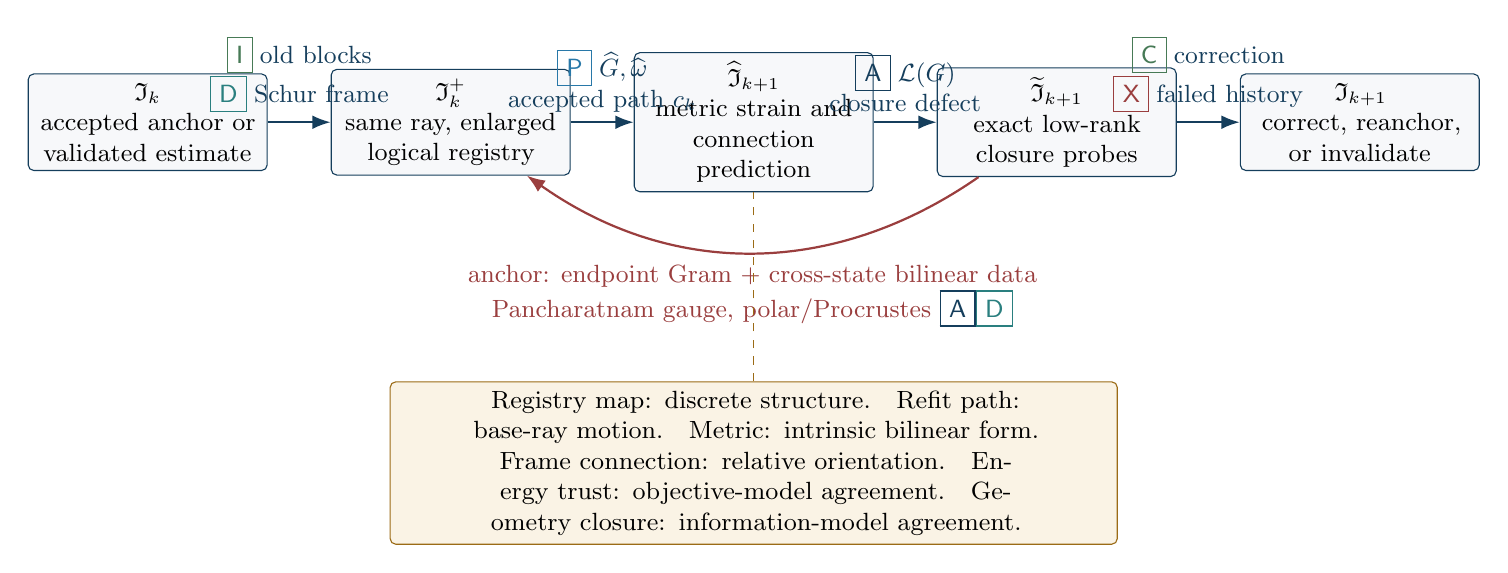
\begin{tikzpicture}[node distance=7mm and 8mm,>=Latex,every node/.style={font=\small},box/.style={draw=navy,rounded corners=2pt,fill=paper,align=center,minimum height=11mm,text width=28mm},arr/.style={->,thick,navy}]
\node[box] (Ik) {$\mathfrak I_k$\\accepted anchor or\\validated estimate};
\node[box,right=of Ik] (grow) {$\mathfrak I_k^+$\\same ray, enlarged\\logical registry};
\node[box,right=of grow] (pred) {$\widehat{\mathfrak I}_{k+1}$\\metric strain and\\connection prediction};
\node[box,right=of pred] (probe) {$\widetilde{\mathfrak I}_{k+1}$\\exact low-rank\\closure probes};
\node[box,right=of probe] (next) {$\mathfrak I_{k+1}$\\correct, reanchor,\\or invalidate};
\draw[arr] (Ik)--node[above,align=center]{\status{green}{I}\;old blocks\\\status{teal}{D}\;Schur frame}(grow);
\draw[arr] (grow)--node[above,align=center]{\status{blue}{P}\;$\widehat G,\widehat\omega$\\accepted path $c_k$}(pred);
\draw[arr] (pred)--node[above,align=center]{\status{navy}{A}\;$\mathcal L(G)$\\closure defect}(probe);
\draw[arr] (probe)--node[above,align=center]{\status{green}{C}\;correction\\\status{red}{X}\;failed history}(next);
\draw[arr,red,bend left=35] (probe) to node[below=1mm,align=center,fill=white,inner sep=1.5pt]{anchor: endpoint Gram + cross-state bilinear data\\Pancharatnam gauge, polar/Procrustes \status{navy}{A}\status{teal}{D}} (grow);
\node[below=24mm of pred,draw=gold,fill=softgold,rounded corners=2pt,align=center,text width=90mm] (types) {Registry map: discrete structure.\quad Refit path: base-ray motion.\quad Metric: intrinsic bilinear form.\\Frame connection: relative orientation.\quad Energy trust: objective-model agreement.\quad Geometry closure: information-model agreement.};
\draw[dashed,gold] (types)--(pred);
\end{tikzpicture}
\caption{One outer adaptive iteration as a typed information recursion.  Status marks are \status{navy}{A} acquired anchor, \status{green}{I} exact inheritance, \status{teal}{D} classical derivation, \status{blue}{P} prediction, \status{green}{C} correction, and \status{red}{X} invalidation.  The lower reanchor arrow activates when closure requests an authoritative anchor.}
\label{fig:global}
\end{figure*}

\section{The global mathematical architecture}

\begin{microbox}
The reusable object is a typed geometric-information tuple: its matrix is paired with a base ray, registry, supported quotient, frame, transformation law, and provenance.  Structural growth and physical motion therefore follow different arrows.
\end{microbox}

Let $\Hh$ be a finite-dimensional complex Hilbert space with inner product conjugate-linear in its first argument and linear in its second.  Normalized vectors differing by phase represent the same physical state,
\begin{equation}
 |\psi\rangle\sim e^{i\varphi}|\psi\rangle,
 \qquad x=[\psi]\in\Pj(\Hh).
 \label{eq:ray}
\end{equation}
A smooth accepted logical chart and its runtime realization form the typed chain
\begin{equation}
 \R^{r_k}\xrightarrow{O_k}\R^{d_k}
 \xrightarrow{J_k}\R^{m_k}
 \xrightarrow{T_{\rt,k}}T_{x_k}\Pj(\Hh),
 \qquad E_k=T_{\rt,k}J_kO_k.
 \label{eq:typedchain}
\end{equation}
The four spaces contain, respectively, supported frame coefficients, accepted logical-coordinate velocities, runtime gate velocities, and physical horizontal tangents.  The tying map $\iota_k:\R^{d_k}\to\R^{m_k}$ has Jacobian $J_k=D\iota_k(\theta_k)$.  Runtime splitting, logical tying, physical Gram-null redundancy, and solver damping are consequently four different operations.

The outer information state will be derived as
\begin{equation}
 \mathfrak I_k=(x_k,\mathcal A_k,\theta_k;\,G_k,O_k,E_k;\,\beta_k,A_k,B_k;\,\widehat{\mathcal S}_k,\widehat\omega_k;\,\mathscr L_k,\chi_k),
 \label{eq:statepreview}
\end{equation}
where $\beta_k$ is the supported energy covector, $A_k$ a direct objective-curvature form, $B_k$ an inverse response, $\widehat{\mathcal S}_k$ a metric-strain predictor, $\widehat\omega_k$ a frame-connection predictor, $\mathscr L_k$ an acquisition ledger, and $\chi_k$ the collection of validity and trust certificates.  Semicolons separate physical state, exact/predicted geometry, objective information, evolution model, and provenance.  No component is meaningful after detaching it from the preceding components.

\begin{litbox}
The projective metric follows Provost and Vall\'ee's Hilbert-space construction \cite{Provost1980}; quantum natural gradient uses its pullback as the descent geometry \cite{Stokes2020}.  Retractions, vector transports, and Riemannian quasi-Newton secants follow the typed framework of Absil, Mahony, and Sepulchre and Huang--Gallivan--Absil \cite{Absil2008,Huang2015,Huang2018}.  The split into an intrinsic metric model and a frame-orientation model is the new synthesis required by outer adaptive reuse.
\end{litbox}

\conceptbreak

\section{Anchored split-connection prediction}
\label{sec:prediction}

\subsection{Why the prediction is split}

The estimator carries two evolution laws.  The first predicts how the pullback ruler changes in the accepted logical chart.  The second predicts how an orthonormal tangent frame rotates between fibers after the ruler has been normalized.  Their separation is forced by \cref{sec:identifiability}.

Let $G(t)$ denote the positive-definite restriction of the logical metric to a fixed supported stratum along a segment of $c_k$.  Its tangent space inside the positive cone consists of symmetric matrices.  A metric-strain predictor is a covariant map
\begin{equation}
 \widehat{\mathcal S}_{\theta}:T_\theta\Theta\longrightarrow\operatorname{Sym}(T_\theta^*\Theta\otimes T_\theta^*\Theta),
 \qquad v\longmapsto\widehat{\mathcal S}_{\theta}[v],
 \label{eq:strainmap}
\end{equation}
trained only from prior anchors, directional metric observations, or differentiated circuit information whose provenance is recorded.  For a microstep $h v$, define the positive prediction by the affine-invariant exponential
\begin{align}
 \widehat G^{+}
 &=\Exp_{\widehat G}\!\left(h\widehat{\mathcal S}_{\theta}[v]\right)\nonumber\\
 &=\widehat G^{1/2}
 \exp\!\left(h\widehat G^{-1/2}\widehat{\mathcal S}_{\theta}[v]\widehat G^{-1/2}\right)
 \widehat G^{1/2}.
 \label{eq:metricexp}
\end{align}
The matrix formula represents the congruence-invariant exponential on the positive cone \cite{Moakher2005}; it yields
\begin{equation}
 \widehat G^+=\widehat G+h\widehat{\mathcal S}_{\theta}[v]+O(h^2)
 \label{eq:metriclocal}
\end{equation}
and preserves positive definiteness without eigenvalue clipping.  On a rank-deficient chart it is applied only to the certified support, while the null-space and rank gates are monitored separately.

Under $\theta=S\phi$ with constant invertible $S$, $v_\theta=Sv_\phi$ and
\begin{equation}
 \widehat G_\phi=S^{\mathsf T}\widehat G_\theta S,\qquad
 \widehat{\mathcal S}_{\phi}[v_\phi]
 =S^{\mathsf T}\widehat{\mathcal S}_{\theta}[Sv_\phi]S.
 \label{eq:straincovariance}
\end{equation}
Congruence invariance of \eqref{eq:metricexp} then gives $\widehat G_\phi^+=S^{\mathsf T}\widehat G_\theta^+S$.  The prediction is therefore covariant under logical rescaling.

\subsection{The metric polar lift}

Given two positive metrics $G_0,G_1$ on the same raw supported coordinate space, define
\begin{equation}
 C_{1,0}=(G_1^{-1}G_0)^{1/2},
 \label{eq:metricpolar}
\end{equation}
where the principal square root is taken as a positive $G_1$-self-adjoint endomorphism.  Since
\begin{equation}
 C_{1,0}^{\mathsf T}G_1=G_1C_{1,0},\qquad C_{1,0}^2=G_1^{-1}G_0,
 \label{eq:selfadjoint}
\end{equation}
one obtains
\begin{equation}
 C_{1,0}^{\mathsf T}G_1C_{1,0}=G_1C_{1,0}^2=G_0.
 \label{eq:polarisometry}
\end{equation}
Thus $C_{1,0}$ is the unique positive $G_1$-self-adjoint isometry from $(\R^r,G_0)$ to $(\R^r,G_1)$.  It is a \emph{minimal-strain identification} induced by the common logical chart, not a recovered physical rotation.  Under \eqref{eq:covariance},
\begin{equation}
 C_{1,0}^{(\phi)}=S^{-1}C_{1,0}^{(\theta)}S,
 \label{eq:polarcovariance}
\end{equation}
because principal square roots respect similarity.  This is the coordinate-covariant alternative to minimizing an unweighted Frobenius distance from the identity, which would privilege a parameter scale.

Let $O_i,L_i$ be exact or predicted support maps satisfying $L_iO_i=\Id_r$.  The polar lift in whitened coefficients is
\begin{equation}
 R^g_{1,0}=L_1C_{1,0}O_0,\qquad (R^g_{1,0})^{\mathsf T}R^g_{1,0}=\Id_r.
 \label{eq:polarcoeff}
\end{equation}
Different spectral gauges for $O_i$ conjugate $R^g_{1,0}$ by orthogonal factors and leave the synthesized raw map unchanged.

\subsection{The skew frame connection}

For a differentiable physical orthonormal frame $E(t)$, define the frame connection along the accepted path by
\begin{equation}
 \omega(t)=\Rea\!\left(E(t)^\dagger\nabla_{\dot x(t)}E(t)\right).
 \label{eq:spinconnection}
\end{equation}
Differentiating $\Rea(E^\dagger E)=\Id$ gives
\begin{equation}
 0=\dot E^\flat E+E^\flat\dot E=\omega^{\mathsf T}+\omega,\qquad \omega\in\mathfrak o(r),
 \label{eq:omegaskew}
\end{equation}
where $\mathfrak o(r)$ is the space of skew-symmetric matrices.  Parallel coefficients solve
\begin{align}
 \dot z(t)+\omega(t)z(t)&=0,\nonumber\\
 R^\omega_{1,0}
 &=\mathcal P\exp\!\left(-\int_0^1\omega(t)\,dt\right)\in O(r).
 \label{eq:pathordered}
\end{align}
The symbol $\mathcal P$ orders noncommuting factors along the path.  Under a time-dependent frame gauge $E'(t)=E(t)Q(t)$,
\begin{equation}
 \omega'=Q^{\mathsf T}\omega Q+Q^{\mathsf T}\dot Q,\qquad
 R^{\omega'}_{1,0}=Q(1)^{\mathsf T}R^\omega_{1,0}Q(0),
 \label{eq:gaugeconnection}
\end{equation}
which is precisely the covariance needed for the physical transported vector to remain unchanged.

The exact $\omega$ requires differentiated tangent data or an exact connection.  The measurement-saving route carries a model $\widehat\omega$ calibrated by prior anchors.  With no orientation history, $\widehat\omega=0$ is the declared minimal-rotation prior; it is not an inference from endpoint metrics.  The one-segment predicted coefficient transport is
\begin{equation}
 \widehat P_{1,0}=\widehat R^\omega_{1,0}\widehat R^g_{1,0},\qquad
 \widehat P_{1,0}^{\mathsf T}\widehat P_{1,0}=\Id_r,
 \label{eq:splittransport}
\end{equation}
and the raw supported transport is
\begin{equation}
 \widehat{\mathsf V}_{1,0}=\widehat O_1\widehat P_{1,0}L_0,\qquad
 \widehat{\mathsf V}_{1,0}^{\mathsf T}\widehat G_1\widehat{\mathsf V}_{1,0}=G_0
 \quad\text{on }\im O_0.
 \label{eq:rawtransport}
\end{equation}

\begin{theorem}[Dominant predictive transport]
On an interval of fixed supported rank, equations \eqref{eq:metricexp} and \eqref{eq:splittransport} define a positive, coordinate-covariant, metric-compatible predictive transport.  If $\widehat{\mathcal S}[\dot\theta]=\dot G+O(h)$ and $\widehat\omega=\omega+O(h)$ over a step of length $h$, then a first-order quadrature produces one-step errors
\begin{align}
 \|G(t+h)-\widehat G(t+h)\|&=O(h^2),\nonumber\\
 \|P(t+h,t)-\widehat P(t+h,t)\|&=O(h^2).
 \label{eq:localorder}
\end{align}
Composition over accepted inner steps gives
\begin{equation}
 \widehat P_{n,0}=\widehat P_{n,n-1}\cdots\widehat P_{1,0}.
 \label{eq:composition}
\end{equation}
At a fixed ray with fixed logical chart, $\widehat{\mathcal S}=0$ and $\widehat\omega=0$ reduce the construction to identity transport.
\end{theorem}

\begin{proof}
Positivity follows from the matrix exponential.  Coordinate covariance follows from \eqref{eq:straincovariance} and \eqref{eq:polarcovariance}; frame-gauge covariance follows from \eqref{eq:gaugeconnection}.  Orthogonality of both factors in \eqref{eq:splittransport} proves metric compatibility through \eqref{eq:rawtransport}.  Taylor expansion of the exponential and the ordered exponential gives local error $O(h^2)$ when their generators have $O(h)$ error.  Product composition is the defining cocycle law for discrete transport.  The fixed-ray statement follows by substitution.
\end{proof}

If only the endpoint displacement $\Delta\theta_k$ is retained, one may use one segment with $v=\Delta\theta_k$.  Retaining accepted inner steps gives a more faithful path integral at no new quantum-estimation cost.  An exact connection supplies authoritative transport without cross-state Procrustes.  A zero-order frozen model $\widehat G_{k+1}=G_k^+$, $\widehat\omega=0$ remains licensed for sufficiently short refits but has only $O(\ell_k)$ error, where
\begin{equation}
 \ell_k=\int_0^1\sqrt{\dot\theta(t)^{\mathsf T}G(t)\dot\theta(t)}\,dt
 \label{eq:pathlength}
\end{equation}
is the Fubini--Study path length.

\begin{litbox}
The affine-invariant positive-cone geometry imports congruence covariance from matrix geometric-mean theory \cite{Moakher2005}.  The connection, retraction, and vector-transport types are standard Riemannian optimization objects \cite{Absil2008,Huang2015}.  The particular split predictor, its anchor calibration, and its use across outer ansatz growth are new here.
\end{litbox}

\subsection{What qBANG does and does not certify}

qBANG and qBroyden initialize a quantum Fisher matrix or its inverse and update it with gradient outer products, using a positive rank-one recurrence and Sherman--Morrison inversion \cite{Fitzek2024}.  In abstract form,
\begin{equation}
 \widehat F^{+}=(1-\alpha)\widehat F+\alpha\,q q^{\mathsf T},\qquad 0<\alpha\le1,
 \label{eq:qbangabstract}
\end{equation}
for a gradient-derived $q$.  Positivity and preconditioning utility are genuine.  Equality to the Fubini--Study metric requires an additional identification theorem relating gradient covariance or a relative-entropy Hessian to quantum Fisher information.  For a deterministic energy gradient at one state, $q q^{\mathsf T}$ is rank one and is not generally the Hilbert-space tangent Gram matrix.  Accordingly, \eqref{eq:qbangabstract} may initialize or regularize $\widehat{\mathcal S}$, but it cannot by itself carry the status \status{navy}{A} of exact geometric evolution.  This limitation is why the closure probes below are indispensable.

\conceptbreak

\section{Deterministic geometric closure}
\label{sec:closure}

\begin{microbox}
A prediction becomes reusable by surviving an exact observation chosen in the directions that matter.  Agreement on a few directions certifies only those directions; agreement on a spanning probe set closes the whole represented metric.
\end{microbox}

Let $\widehat G$ be the endpoint prediction on rank $r$ support and let $\widehat O$ satisfy $\widehat O^{\mathsf T}\widehat G\widehat O=\Id_r$.  The true relative error in the predicted frame is
\begin{equation}
 D=\widehat O^{\mathsf T}(G-\widehat G)\widehat O\in\operatorname{Sym}(r).
 \label{eq:relativeerror}
\end{equation}
Choose a probe coefficient matrix $X\in\R^{r\times q}$ and prepare raw logical directions $Z=\widehat OX$.  Exact same-state tangent acquisition gives
\begin{align}
 Y&=Z^{\mathsf T}GZ=X^{\mathsf T}(\Id_r+D)X,\nonumber\\
 \widehat Y&=Z^{\mathsf T}\widehat GZ=X^{\mathsf T}X,\nonumber\\
 R&=Y-\widehat Y=X^{\mathsf T}DX.
 \label{eq:probeobservation}
\end{align}
For full-column-rank $X$, define the dimensionless closure defect
\begin{equation}
 \delta_X=\left\|\widehat Y^{-1/2}R\widehat Y^{-1/2}\right\|_{\op}.
 \label{eq:closuredefect}
\end{equation}
This compares exact and predicted squared Fubini--Study lengths in the probed subspace, so it is invariant under a change of probe basis $X\mapsto XR$.

More general acquired quantities---individual Gram entries, active--candidate overlaps, or polarized mixed bilinears---are represented by a linear observation operator
\begin{equation}
 \mathcal L:\operatorname{Sym}(r)\to\R^s,\qquad
 y=\mathcal L(D).
 \label{eq:linearobservation}
\end{equation}
Candidate--active overlaps test the mixed blocks actually observed; they do not close an unseen active--active block unless the resulting $\mathcal L$ is injective on the admissible error space.

\begin{theorem}[Deterministic geometric closure]
For the quadratic probe \eqref{eq:probeobservation}:
\begin{enumerate}[label=(\roman*)]
\item If $\delta_X\le\varepsilon<1$, then for every $a\in\R^q$,
\begin{equation}
 (1-\varepsilon)a^{\mathsf T}\widehat Ya
 \le a^{\mathsf T}Ya
 \le(1+\varepsilon)a^{\mathsf T}\widehat Ya.
 \label{eq:probebound}
\end{equation}
\item If $X$ has full row rank $r$ and the observations are consistent, then
\begin{equation}
 D=(X^+)^{\mathsf T}RX^+,\qquad
 \|D\|_{\op}\le\|X^+\|_{\op}^2\|R\|_{\op}.
 \label{eq:fullreconstruction}
\end{equation}
Thus $R=0$ certifies $G=\widehat G$ on the represented support.
\item If $\rank X=q<r$, $R=0$ certifies only the compression of $D$ to $\im X$.  Errors mapping or living entirely in $(\im X)^\perp$ remain unidentified.
\item For a general linear observation, zero defect certifies the full admissible error exactly when $\ker\mathcal L$ intersects that error class only at zero.
\end{enumerate}
\end{theorem}

\begin{proof}
The definition \eqref{eq:closuredefect} is equivalent to
\begin{equation}
 -\varepsilon\Id_q\preceq\widehat Y^{-1/2}R\widehat Y^{-1/2}\preceq\varepsilon\Id_q,
\end{equation}
and congruence by $\widehat Y^{1/2}$ gives \eqref{eq:probebound}.  If $X$ has full row rank, $XX^+=\Id_r$; multiplying $R=X^{\mathsf T}DX$ by $(X^+)^{\mathsf T}$ and $X^+$ gives \eqref{eq:fullreconstruction}.  If $X$ is not spanning, take any nonzero symmetric $D$ supported on $(\im X)^\perp$ to obtain $X^{\mathsf T}DX=0$.  The last statement is the definition of injectivity on a model class.
\end{proof}

\subsection{Minimum-change correction and escalation}

When a probe fails the continuation tolerance but remains support-compatible, correct the prediction in its own whitened frame.  The minimum-Frobenius correction for a consistent quadratic probe is
\begin{equation}
 \Delta_X=(X^+)^{\mathsf T}RX^+,\qquad
 \widehat G^{\Cor}=\widehat L^{\mathsf T}(\Id_r+\Delta_X)\widehat L.
 \label{eq:mincorrection}
\end{equation}
Here $\widehat L$ is the analysis map of the predicted supported factorization,
$\widehat G=\widehat L^{\mathsf T}\widehat L$ and
$\widehat L\widehat O=\Id_r$.  This form is well typed even when the raw Gram
matrix is singular; no inverse of the rectangular synthesis map $\widehat O$
is implied.
For a general observation, the Hilbert-space projection formula is
\begin{equation}
 \Delta=\mathcal L^*(\mathcal L\mathcal L^*)^+y,
 \label{eq:operatorcorrection}
\end{equation}
where $\mathcal L^*$ is the Frobenius adjoint.  It is the smallest symmetric correction satisfying the acquired constraints.  It is accepted only if
\begin{align}
 \lambda_{\min}(\Id_r+\Delta)&>\tau_c,\nonumber\\
 \|\Delta\|_{\op}&\le\varepsilon_c,\nonumber\\
 \dist(\im\widehat O,\im O^{\Cor})&\le\varepsilon_s.
 \label{eq:correctiongate}
\end{align}
The first gate preserves positive support, the second limits unobserved extrapolation, and the third protects the support subspace.  Davis--Kahan and Wedin perturbation bounds relate the last gate to a spectral gap \cite{DavisKahan1970,Wedin1972}.

The event-driven decision rule is
\begin{equation}
 \mathcal G=
 \begin{cases}
 \Prd,&\delta_X\le\varepsilon_p,\ \text{stable gap},\\
 \Cor,&\delta_X\le\varepsilon_c,\ \eqref{eq:correctiongate},\\
 \A,&\mathcal L\ \text{not diagnostic},\\
 \Inv,&\text{rank/correction failure}.
 \end{cases}
 \label{eq:escalation}
\end{equation}
The $\A$ branch first acquires the smallest block that makes the relevant observation injective.  If closure still fails, it acquires the full endpoint metric; if orientation confidence also fails, it acquires cross-state tangent data and performs the anchor registration of \cref{sec:procrustes}.  Curvature history attached to rejected support is quarantined until a new common-support certificate authorizes reuse.

\begin{figure}[t]
\centering
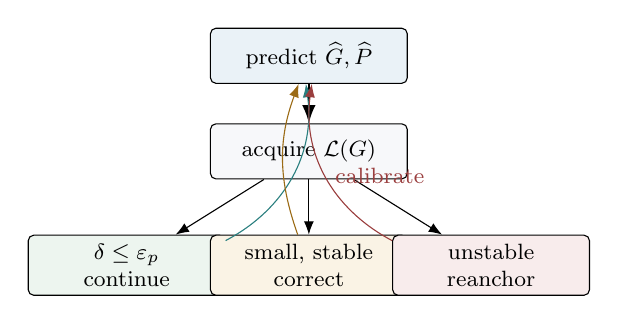
\begin{tikzpicture}[node distance=5mm,>=Latex,every node/.style={font=\footnotesize},n/.style={draw,rounded corners=2pt,align=center,minimum width=25mm,minimum height=7mm}]
\node[n,fill=softblue] (p) {predict $\widehat G,\widehat P$};
\node[n,fill=paper,below=of p] (o) {acquire $\mathcal L(G)$};
\node[n,fill=softgreen,below left=7mm and -2mm of o] (c) {$\delta\le\varepsilon_p$\\continue};
\node[n,fill=softgold,below=7mm of o] (u) {small, stable\\correct};
\node[n,fill=softred,below right=7mm and -2mm of o] (a) {unstable\\reanchor};
\draw[->,thick] (p)--(o);
\draw[->] (o)--(c);\draw[->] (o)--(u);\draw[->] (o)--(a);
\draw[->,teal,bend right=35] (c) to (p);
\draw[->,gold,bend left=20] (u) to (p);
\draw[->,red,bend left=35] (a) to node[right]{calibrate} (p);
\end{tikzpicture}
\caption{Geometric confidence is closed by falsifiable observations, and a failed information model triggers reanchoring.}
\label{fig:closurecycle}
\end{figure}

\subsection{Sensitivity of downstream quantities}

Assume a complete relative bound
\begin{equation}
 \varepsilon=\|D\|_{\op}<1.
 \label{eq:epsiloncomplete}
\end{equation}
Then
\begin{align}
 (1-\varepsilon)\widehat G&\preceq G\preceq(1+\varepsilon)\widehat G,
 \label{eq:metricorder}\\
 \left|\frac{\|u\|_G}{\|u\|_{\widehat G}}-1\right|
 &\le\max\{\sqrt{1+\varepsilon}-1,1-\sqrt{1-\varepsilon}\},
 \label{eq:normsensitivity}\\
 \|G^{-1}-\widehat G^{-1}\|_{\widehat G}
 &\le\frac{\varepsilon}{1-\varepsilon}.
 \label{eq:inversesensitivity}
\end{align}
For a natural-gradient or metric-preconditioned direction $p=-G^{-1}b$ and $\widehat p=-\widehat G^{-1}b$,
\begin{equation}
 \|p-\widehat p\|_{\widehat G}
 \le\frac{\varepsilon}{1-\varepsilon}\|\widehat p\|_{\widehat G}.
 \label{eq:stepsensitivity}
\end{equation}
If the raw support eigenvalue cluster is separated from the rejection threshold by gap $g>0$, a Gram perturbation $\Delta G$ obeys the schematic subspace bound
\begin{equation}
 \|\sin\Theta(P_+,\widehat P_+)\|_{\op}
 \le\frac{\|\Delta G\|_{\op}}{g}.
 \label{eq:daviskahan}
\end{equation}
Transported gradients and secants inherit both the frame error and \eqref{eq:inversesensitivity}; hence quasi-Newton updates are admitted only after the geometry gate.  Trust radii measured with $\widehat G$ incur \eqref{eq:normsensitivity}.  These bounds assign each tolerance in \eqref{eq:escalation} to the downstream error it controls.

\conceptbreak

\section{Pancharatnam gauge and Procrustes anchors}
\label{sec:procrustes}

\begin{microbox}
The singular-value decomposition is classical.  The cross-state tangent bilinears entering it are new physical information.  Procrustes therefore belongs at an anchor or calibration event, not inside a supposedly measurement-free prediction step.
\end{microbox}

Cross-state Hilbert inner products require a phase convention.  If $\langle\psi_1|\psi_0\rangle\ne0$, choose
\begin{equation}
 \chi=\arg\langle\psi_1|\psi_0\rangle,\qquad
 |\psi_1'\rangle=e^{i\chi}|\psi_1\rangle,\qquad
 \langle\psi_1'|\psi_0\rangle>0.
 \label{eq:pancharatnam}
\end{equation}
Endpoint tangents transform by the same phase.  This is the local Pancharatnam convention \cite{Pancharatnam1956}; a pathwise horizontal lift supplies a phase when the endpoint overlap vanishes or when path holonomy matters \cite{Berry1984,Simon1983}.  With raw horizontal tangent maps $T_0,T_1$ and whiteners $O_0,O_1$, the acquired cross-state block and supported overlap are
\begin{align}
 C_{1,0}&=\Rea\!\left(e^{-i\chi}T_1^\dagger T_0\right),\nonumber\\
 K_{1,0}&=\Rea\!\left((e^{i\chi}E_1)^\dagger E_0\right)
 =O_1^{\mathsf T}C_{1,0}O_0.
 \label{eq:crossraw}
\end{align}
Thus $d_1d_0$ raw cross bilinears or a supported equivalent must be acquired unless circuit structure reduces them.  Endpoint Gram matrices do not generate $C_{1,0}$ classically.

For equal ranks, choose the endpoint frame gauge closest to the source under this declared ambient comparison:
\begin{equation}
 Q_\star\in\arg\min_{Q\in O(r)}
 \|e^{i\chi}E_1Q-E_0\|_{\FS,F}^2.
 \label{eq:procrustesproblem}
\end{equation}
Because both frames are orthonormal,
\begin{align}
 \|e^{i\chi}E_1Q-E_0\|_{\FS,F}^2
 &=2r-2\tr(Q^{\mathsf T}K_{1,0}).
 \label{eq:procrustesexpand}
\end{align}
Let $K_{1,0}=U\Sigma V^{\mathsf T}$ be a singular-value decomposition.  Von Neumann's trace inequality gives
\begin{equation}
 \tr(Q^{\mathsf T}K_{1,0})\le\tr\Sigma,\qquad
 Q_\star=UV^{\mathsf T}.
 \label{eq:procrustessolution}
\end{equation}
This is the orthogonal polar factor derived by Sch\"onemann \cite{Schonemann1966}; stable polar computation and its best-approximation property are developed by Higham \cite{Higham1986}.  The singular values are cosines of principal angles under the chosen comparison.  Small singular values indicate subspace change that no gauge rotation can remove.

For $r_1\ne r_0$, the thin singular value decomposition
\begin{equation}
 K_{1,0}=U_q\Sigma_qV_q^{\mathsf T}+U_\perp\Sigma_\perp V_\perp^{\mathsf T}
 \label{eq:rectsvd}
\end{equation}
is truncated at a registration threshold $\tau_K$.  The partial polar factor
\begin{equation}
 Q_q=U_qV_q^{\mathsf T},\qquad
 Q_q^{\mathsf T}Q_q=V_qV_q^{\mathsf T},\qquad
 Q_qQ_q^{\mathsf T}=U_qU_q^{\mathsf T}
 \label{eq:partialpolar}
\end{equation}
is an isometry only between the common source and target subspaces.  Target directions orthogonal to $U_q$ are new; source directions orthogonal to $V_q$ are lost.  Curvature attached to the latter is quarantined.

\begin{proposition}[Role of an anchor registration]
The Procrustes factor $Q_\star$ is an authoritative \status{teal}{D} gauge registration conditional on the acquired \status{navy}{A} cross block and the phase convention.  It performs three legitimate tasks:
\begin{align}
 R_k&=Q_\star\widehat P_{1,0}^{\mathsf T},\nonumber\\
 \widehat P_{1,0}&\leftarrow Q_\star,\nonumber\\
 \widehat\omega&\leftarrow
 \operatorname{Update}(\widehat\omega,\Log R_k,c_k).
 \label{eq:anchorcalibration}
\end{align}
It measures the residual transition, replaces a failed predicted transition for the committed anchor, and calibrates the future connection model.  It does not follow from endpoint metrics, and chordal endpoint registration is not automatically identical to Levi--Civita parallel transport along the actual refit path.
\end{proposition}

For sufficiently short paths, the principal logarithm $\Log R_k\in\mathfrak o(r)$ is an integrated connection residual.  When an eigenvalue of $R_k$ approaches $-1$, the logarithm branch is unstable; the anchor remains valid, but a unique averaged connection update is not identifiable.  This is an explicit calibration gate.

\begin{figure}[t]
\centering
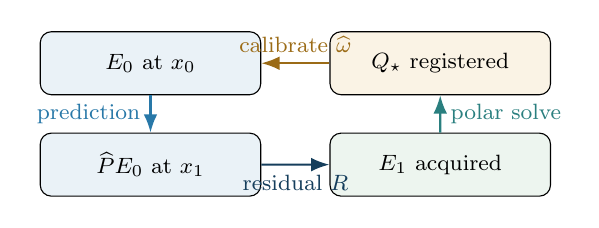
\begin{tikzpicture}[>=Latex,every node/.style={font=\footnotesize},scale=.92]
\node[draw,rounded corners,fill=softblue,minimum width=28mm,minimum height=8mm] (s) at (0,0) {$E_0$ at $x_0$};
\node[draw,rounded corners,fill=softblue,minimum width=28mm,minimum height=8mm] (p) at (0,-1.4) {$\widehat P E_0$ at $x_1$};
\node[draw,rounded corners,fill=softgreen,minimum width=28mm,minimum height=8mm] (e) at (4,-1.4) {$E_1$ acquired};
\node[draw,rounded corners,fill=softgold,minimum width=28mm,minimum height=8mm] (q) at (4,0) {$Q_\star$ registered};
\draw[->,thick,blue] (s)--node[left]{prediction}(p);
\draw[->,thick,navy] (p)--node[below]{residual $R$}(e);
\draw[->,thick,teal] (e)--node[right]{polar solve}(q);
\draw[->,thick,gold] (q)--node[above]{calibrate $\widehat\omega$}(s);
\end{tikzpicture}
\caption{The reanchor cycle.  Cross-state acquisition closes the orientation ambiguity and returns a residual used to train, not retroactively justify, the predictor.}
\label{fig:reanchor}
\end{figure}

\conceptbreak

\section{Projective support and exact whitening}
\label{sec:support}

\subsection{Horizontal tangents and the real pullback metric}

At a normalized representative $|\psi(\theta)\rangle$, phase is removed by
\begin{equation}
 \Pi_\psi=\Id-|\psi\rangle\langle\psi|,
 \qquad |t_a\rangle=\Pi_\psi|\partial_a\psi\rangle.
 \label{eq:horizontal}
\end{equation}
The logical tangent synthesis map $T:\R^d\to T_x\Pj(\Hh)$ and its real analysis map $T^\flat$ are
\begin{align}
 Tu&=\sum_{a=1}^d u^a|t_a\rangle,\nonumber\\
 T^\flat|\xi\rangle&=\Rea(T^\dagger|\xi\rangle),
 \qquad G=T^\flat T=\Rea(T^\dagger T).
 \label{eq:synthesisanalysis}
\end{align}
Here $G$ is the real symmetric positive-semidefinite bilinear form induced on raw parameter coordinates by the tangent map.  Direct substitution gives
\begin{align}
 u^{\mathsf T}Gu
 &=u^{\mathsf T}\Rea(T^\dagger T)u
 =\Rea\langle Tu|Tu\rangle
 =\|Tu\|_{\FS}^2,\nonumber\\
 u\in\ker G
 &\Longleftrightarrow u^{\mathsf T}Gu=0
 \Longleftrightarrow Tu=0,
 \qquad \ker G=\ker T.
 \label{eq:kernel}
\end{align}
Thus the represented physical tangent space is the quotient $\R^d/\ker G$.  A quotient identifies coordinate vectors whose difference synthesizes no first-order ray motion.

\begin{theorem}[Projective supported-frame theorem]
Let $G=V_+\Lambda_+V_+^{\mathsf T}$ contain precisely the eigenvalues $\lambda_i>\tau_G$, with $V_+^{\mathsf T}V_+=\Id_r$.  Define
\begin{equation}
 O=V_+\Lambda_+^{-1/2},\quad
 L=\Lambda_+^{1/2}V_+^{\mathsf T},\quad
 E=TO.
 \label{eq:whitening}
\end{equation}
Then $O:\R^r\to\im V_+$ synthesizes supported raw coordinates, $L:\R^d\to\R^r$ analyzes the represented quotient, and
\begin{align}
 LO&=\Id_r,\qquad OL=V_+V_+^{\mathsf T}=P_+,\nonumber\\
 O^{\mathsf T}GO&=\Id_r,\qquad \Rea(E^\dagger E)=\Id_r,\nonumber\\
 Tu&=ELu\quad(u\in\im V_+),\nonumber\\
 \|ELu\|_{\FS}^2&=u^{\mathsf T}Gu.
 \label{eq:frameidentities}
\end{align}
The Moore--Penrose inverse is $G^+=O O^{\mathsf T}=V_+\Lambda_+^{-1}V_+^{\mathsf T}$ on certified support.
\end{theorem}

\begin{proof}
Every identity follows without an untyped inverse:
\begin{align}
 LO&=\Lambda_+^{1/2}V_+^{\mathsf T}V_+\Lambda_+^{-1/2}=\Id_r,\nonumber\\
 OL&=V_+\Lambda_+^{-1/2}\Lambda_+^{1/2}V_+^{\mathsf T}=P_+,\nonumber\\
 O^{\mathsf T}GO
 &=\Lambda_+^{-1/2}V_+^{\mathsf T}
   V_+\Lambda_+V_+^{\mathsf T}V_+\Lambda_+^{-1/2}=\Id_r,\nonumber\\
 \Rea(E^\dagger E)&=O^{\mathsf T}\Rea(T^\dagger T)O=\Id_r.
\end{align}
For $u=P_+u$, $OLu=u$ and $ELu=TOLu=Tu$.  Null components are deliberately excluded, not damped into artificial physical modes.
\end{proof}

The solver may use
\begin{equation}
 W=V_+(\Lambda_++\mu\Id_r)^{-1/2},\qquad \mu>0,
 \label{eq:ridge}
\end{equation}
but $TW$ is not the exact orthonormal frame unless $\mu=0$.  The threshold $\tau_G$ decides physical support; $\mu$ changes numerical response only after that decision.

\subsection{Vectors, covectors, and coordinate covariance}

The energy differential $b=dE_\theta\in(\R^d)^*$ pairs with a coordinate displacement as $b[u]=b^{\mathsf T}u$.  Its supported representation is
\begin{equation}
 \beta=O^{\mathsf T}b,\qquad b[P_+u]=\beta^{\mathsf T}Lu.
 \label{eq:covectoranalysis}
\end{equation}
Under an invertible linear reparameterization $\theta=S\phi$,
\begin{align}
 T_\phi&=T_\theta S,&
 G_\phi&=S^{\mathsf T}G_\theta S,\nonumber\\
 b_\phi&=S^{\mathsf T}b_\theta,&
 u_\theta&=Su_\phi,
 \label{eq:covariance}
\end{align}
and therefore
\begin{align}
 T_\phi u_\phi&=T_\theta u_\theta,\nonumber\\
 u_\phi^{\mathsf T}G_\phi u_\phi&=u_\theta^{\mathsf T}G_\theta u_\theta,\nonumber\\
 b_\phi^{\mathsf T}u_\phi&=b_\theta^{\mathsf T}u_\theta.
 \label{eq:invariants}
\end{align}
Whitening frames constructed independently in the two charts can differ by an orthogonal gauge $R\in O(r)$, but the physical frame and every synthesized update agree after $z_\phi=Rz_\theta$.  Hence coordinate covariance consists of transforming the quotient, vectors, covectors, and bilinear forms together; raw matrix entries may vary while the physical invariants in \eqref{eq:invariants} agree.

\begin{physbox}
$G$ answers ``how far does the ray move?''; $b$ answers ``how does energy pair with that move?''; $A$ answers ``how does that pairing change?''  Exact whitening turns the first question into Euclidean length without conflating the three objects.
\end{physbox}

\conceptbreak

\section{The SR projected-logical route}
\label{sec:sr}

Let $\Psi_{\rt}:\R^m\to\Pj(\Hh)$ be the runtime circuit and $\iota:\R^d\to\R^m$ the smooth tying map.  The accepted logical manifold is
\begin{equation}
 \Psi=\Psi_{\rt}\circ\iota,\qquad
 T=T_{\rt}J_\iota,\qquad
 G=J_\iota^{\mathsf T}G_{\rt}J_\iota.
 \label{eq:logicalpullback}
\end{equation}
For a logical velocity $u$, the equality
\begin{equation}
 \|T_{\rt}J_\iota u\|_{\FS}^2
 =u^{\mathsf T}J_\iota^{\mathsf T}G_{\rt}J_\iota u
 =u^{\mathsf T}Gu
 \label{eq:logicalinvariant}
\end{equation}
shows why runtime redundancy must be projected before physical support is interpreted.  The full accepted-ansatz refit searches the positive support of this logical $G$.  A selector window $W\subset\{1,\ldots,d\}$ supplies only the blocks it actually measures; it is not the complete persistent chart.

Suppose a candidate response calculation uses a compensated tangent block
\begin{equation}
 T_B^\star=T_B+T_WR,\qquad R:\R^p\to\R^{|W|}.
 \label{eq:compensated}
\end{equation}
This corresponds to the coordinate injection $\alpha\mapsto(R\alpha,\alpha)$ used during conditional relaxation.  Structural admission instead adds the raw coordinate injection $\alpha\mapsto(0,\alpha)$.  The two are related, not interchangeable:
\begin{align}
 T_B&=T_B^\star-T_WR,\nonumber\\
 G_{EB}&=G_{EB}^\star-G_{EW}R,\nonumber\\
 G_{BB}&=G_{BB}^\star-R^{\mathsf T}G_{WB}^\star
 -G_{BW}^\star R+R^{\mathsf T}G_{WW}R.
 \label{eq:decompensate}
\end{align}
Here $G_{EB}=\Rea(E^\dagger T_B)$ and similarly for the other blocks.  Equation~\eqref{eq:decompensate} is a classical congruence once $R$ and the displayed blocks are known.  A window cache lacking $G_{EB}$ for inherited directions outside $W$ does not close the full-chart extension.

\begin{geombox}
The selector may slide a candidate arrow along a small old-coordinate window before judging it.  Admission installs the unslid generator axis.  Decompensation subtracts the slide before the new axis is joined to the complete accepted frame.
\end{geombox}

\conceptbreak

\section{Exact same-ray structural growth}
\label{sec:growth}

\begin{microbox}
At zero amplitude the new gates are identities.  The base ray, old tangent map, old metric block, old differential, and old--old objective curvature are therefore inherited exactly.  Only bilinear information involving genuinely new tangents can be missing.
\end{microbox}

Let $p$ logical directions be admitted at
\begin{equation}
 j_k:\R^{d_k}\hookrightarrow\R^{d_k+p},\qquad
 j_k(\theta)=(\theta,0),\qquad x_k^+=x_k.
 \label{eq:registryembedding}
\end{equation}
For the ordered product ansatz with identity new factors,
\begin{equation}
 \Psi_{k+1}(\theta,0)=\Psi_k(\theta)
 \label{eq:restrictionidentity}
\end{equation}
in a neighborhood of $\theta_k$ along the old coordinates.  Differentiating the restriction once and twice yields
\begin{align}
 T_D^+&=T_k,&G_{DD}^+&=G_k,&b_D^+&=b_k,&A_{DD}^+&=A_k,
 \label{eq:oldinherit}
\end{align}
where $D$ denotes the embedded old registry.  These are \status{green}{I} identities.  They do not predict their values after the subsequent refit.

Let $C=T_B:\R^p\to T_{x_k}\Pj(\Hh)$ be the raw admitted tangent block and let $E=E_k$ be the inherited orthonormal physical frame.  Define
\begin{align}
 K&=\Rea(E^\dagger C)=O_k^{\mathsf T}G_{DB},\nonumber\\
 C_\perp&=(\Id-\mathcal P_E)C=C-EK,\nonumber\\
 \Gamma&=\Rea(C_\perp^\dagger C_\perp)
 =G_{BB}-K^{\mathsf T}K,
 \label{eq:residualgrowth}
\end{align}
where $\mathcal P_E\xi=E\Rea(E^\dagger\xi)$ is the real Fubini--Study projector.  If
\begin{equation}
 \Gamma=U_+\Sigma_+U_+^{\mathsf T},\qquad \sigma_i>\tau_G,
 \label{eq:gammaeig}
\end{equation}
then the residual new frame is
\begin{equation}
 F=C_\perp U_+\Sigma_+^{-1/2}.
 \label{eq:newframe}
\end{equation}

\begin{theorem}[Exact same-ray growth and information closure]
Given the authoritative inherited frame $(T_D,G_{DD},O_k,E)$, the enlarged physical support is constructed exactly from the $rp$ real cross bilinears $K=\Rea(E^\dagger C)$ and the $p(p+1)/2$ symmetric elements of $G_{BB}=\Rea(C^\dagger C)$.  The frame
\begin{equation}
 E^+=(E,F),\qquad
 O^+=
 \begin{pmatrix}
 O_k&-O_kKU_+\Sigma_+^{-1/2}\\
 0&U_+\Sigma_+^{-1/2}
 \end{pmatrix}
 \label{eq:extendedwhitener}
\end{equation}
satisfies $E^+=T^+O^+$ and $\Rea((E^+)^\dagger E^+)=\Id_{r+q}$, where $q=\rank_{\tau_G}\Gamma$.  No old--old Gram element is reacquired.  Any cached data that algebraically determine $K$ and $G_{BB}$ reduce this acquisition set; a restricted-window cache is closed precisely when it also determines candidate overlaps with the inherited support orthogonal to that window.
\end{theorem}

\begin{proof}
First,
\begin{align}
 \Rea(E^\dagger C_\perp)&=K-K=0,\nonumber\\
 \Rea(F^\dagger F)
 &=\Sigma_+^{-1/2}U_+^{\mathsf T}\Gamma U_+\Sigma_+^{-1/2}=\Id_q.
\end{align}
Thus $(E,F)$ is orthonormal.  Moreover,
\begin{align}
 T^+O^+
 &=(T_D,C)
 \begin{pmatrix}
 O_k&-O_kKU_+\Sigma_+^{-1/2}\\
 0&U_+\Sigma_+^{-1/2}
 \end{pmatrix}\nonumber\\
 &=\bigl(E,(C-EK)U_+\Sigma_+^{-1/2}\bigr)=(E,F).
\end{align}
Because $E$ spans the full old support, $K$ contains every cross bilinear needed to project $C$ modulo that support.  Conversely, changing an unmeasured entry of $K$ while holding window data fixed changes $\Gamma$ and can change its rank, so the missing overlap is logically necessary.  Under an invertible old-coordinate reparameterization, $E$ changes only by orthogonal gauge and $K^{\mathsf T}K$, $\Gamma$, and the physical residual span remain invariant.
\end{proof}

For one admitted direction $c$, $\gamma=\langle c,c\rangle_{\FS}-\|\Rea(E^\dagger c)\|_2^2$.  If $\gamma>\tau_G$, $f=(c-EK)/\sqrt\gamma$ is one new physical direction; if $\gamma\le\tau_G$, the admitted coordinate is Gram-null modulo the old support and adds no frame dimension.

Objective curvature has the same exact old--old inheritance but a different extension rule.  Before refit one may write, in the new whitened frame,
\begin{equation}
 A_k^+=
 \begin{pmatrix}A_k&A_{kn}\\A_{nk}&A_{nn}\end{pmatrix},\qquad
 B_k^+=
 \begin{pmatrix}\widetilde B_k&B_{kn}\\B_{nk}&B_{nn}\end{pmatrix}.
 \label{eq:curvatureextension}
\end{equation}
Measured candidate Hessian blocks, after the same raw-to-frame congruence as $O^+$, are \status{navy}{A} authoritative on their measured subspace.  The direct-curvature restriction $A_k$ is inherited exactly.  By contrast, setting $\widetilde B_k=B_k$ recycles the old inverse response as a prior; it is the exact old principal block of $(A_k^+)^{-1}$ only when the mixed blocks vanish or their Schur correction has been included.  Unmeasured cross blocks and new-mode diagonals are priors \status{blue}{P}; the neutral positive inverse prior is $B_{nn}=\alpha\Id_q$, $B_{kn}=0$, not an asserted exact Hessian.  This refines the identity extension used in Hessian recycling \cite{Ramoa2025}: direct old curvature is exact at the same ray as a coordinate restriction, whereas inverse-response extension and all new blocks remain explicitly epistemic.

\begin{figure}[t]
\centering
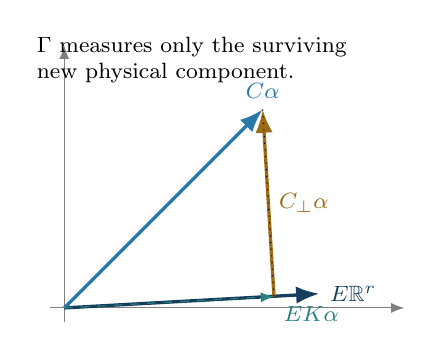
\begin{tikzpicture}[scale=.9,>=Latex,every node/.style={font=\footnotesize}]
\draw[->,gray] (-.2,0)--(4.8,0);
\draw[->,gray] (0,-.2)--(0,3.7);
\draw[very thick,navy,->] (0,0)--(3.6,.2) node[right] {$E\R^r$};
\draw[very thick,blue,->] (0,0)--(2.8,2.8) node[above] {$C\alpha$};
\draw[dashed,teal,->] (0,0)--(2.96,.16) node[below right] {$EK\alpha$};
\draw[very thick,gold,->] (2.96,.16)--(2.8,2.8) node[midway,right] {$C_\perp\alpha$};
\draw[dotted] (2.8,2.8)--(2.96,.16);
\node[align=left] at (1.8,3.5) {$\Gamma$ measures only the surviving\\new physical component.};
\end{tikzpicture}
\caption{Exact frame extension at the unchanged ray.  Candidate projection and Gram--Schur complementation are the same operation in physical and coordinate language.}
\label{fig:growth}
\end{figure}

\conceptbreak

\section{Why endpoint metrics do not transport frames}
\label{sec:identifiability}

After the full accepted-ansatz refit,
\begin{equation}
 c_k:[0,1]\to\Theta_{d_{k+1}},\qquad
 c_k(0)=\theta_k^+,\quad c_k(1)=\theta_{k+1},
 \label{eq:refitpath}
\end{equation}
the base ray changes from $x_k$ to $x_{k+1}$.  Hence $T_{x_k}\M$ and $T_{x_{k+1}}\M$ are different vector spaces.  A metric supplies inner products inside each fiber; a connection supplies comparisons between fibers.

\begin{definition}[Connection and vector transport]
A connection $\nabla$ differentiates tangent vector fields and defines parallel transport $\mathcal T_{t\leftarrow s}:T_{x(s)}\M\to T_{x(t)}\M$ along a path by $\nabla_{\dot x}\xi=0$.  A discrete vector transport is a computable map associated with a retraction step that approximates such a fiber map.  Metric compatibility means
\begin{equation}
 g_{x(t)}(\mathcal T_{t\leftarrow s}\xi,\mathcal T_{t\leftarrow s}\zeta)
 =g_{x(s)}(\xi,\zeta).
 \label{eq:metriccompat}
\end{equation}
\end{definition}

\begin{proposition}[Inter-state non-identifiability]
The source and endpoint pullback metrics $G_0,G_1$, their supported ranks, and a coordinate displacement do not determine the relative physical orientation of the supported frames, their cross overlap, or a parallel transport between them.  Cross-state tangent bilinears, differentiated embedding data, or a declared connection model add information not contained in the endpoint metrics.
\end{proposition}

\begin{proof}
Let $T_1:\R^r\to\psi_1^\perp$ be an endpoint horizontal tangent map.  Any ambient unitary $U$ satisfying $U|\psi_1\rangle=|\psi_1\rangle$ acts unitarily on $\psi_1^\perp$.  Set $\widetilde T_1=UT_1$.  Then
\begin{equation}
 \Rea(\widetilde T_1^\dagger\widetilde T_1)
 =\Rea(T_1^\dagger U^\dagger UT_1)=G_1,
 \label{eq:stabilizer}
\end{equation}
so the endpoint ray and metric are unchanged.  Yet for a source frame $E_0$,
\begin{equation}
 \Rea(\widetilde T_1^\dagger E_0)
 =\Rea(T_1^\dagger U^\dagger E_0)
 \label{eq:crosschanges}
\end{equation}
varies with $U$ whenever the horizontal ambient dimension exceeds the represented rank.  Equivalently, on the frame bundle $E_1$ and $E_1R$, $R\in O(r)$, induce the same endpoint metric but different registrations.  A coordinate displacement constrains the path in the parameter chart, not the unobserved stabilizer action.  Therefore no function of endpoint metrics and displacement alone can recover the cross-frame orientation for all embeddings.
\end{proof}

\begin{physbox}
Two tangent laboratories can each possess a perfectly calibrated ruler while their axes are rotated relative to one another.  $G_0$ and $G_1$ calibrate the rulers.  A connection or a cross-state experiment calibrates the relative axes.
\end{physbox}

The full metric field along a path determines its Levi--Civita connection intrinsically through Christoffel symbols,
\begin{align}
 \Gamma^a{}_{bc}
 &=\frac12G^{ad}
 (\partial_bG_{dc}+\partial_cG_{db}-\partial_dG_{bc}),\nonumber\\
 \dot v^a+\Gamma^a{}_{bc}\dot\theta^b v^c&=0,
 \label{eq:christoffel}
\end{align}
on nonsingular support.  Endpoint values alone do not supply the derivatives or the path integral.  Moreover, intrinsic Levi--Civita transport does not determine the extrinsic bending of an embedded tangent subspace in $\Hh$; the second fundamental form carries that additional information.  The dominant estimator will therefore predict intrinsic strain and frame rotation separately, then test each on the subspace actually observed.

\conceptbreak

\section{Outer secants and objective-curvature reuse}
\label{sec:curvature}

\subsection{Transport laws from invariant pairings}

Let $P:\R^{r_0}\to\R^{r_1}$ be an invertible square coefficient transport on a fixed-rank interval,
\begin{equation}
 z_1=Pz_0.
 \label{eq:vectormap}
\end{equation}
A covector $\gamma_i\in(\R^{r_i})^*$ must preserve its pairing with the same represented physical vector:
\begin{align}
 \gamma_1^{\mathsf T}z_1&=\gamma_0^{\mathsf T}z_0
 =\gamma_0^{\mathsf T}P^{-1}z_1
 \quad\forall z_1,\nonumber\\
 \gamma_1&=P^{-\mathsf T}\gamma_0.
 \label{eq:dualmap}
\end{align}
If $P$ is orthogonal, vectors and covector component columns both transform by $P$, but this is a consequence of orthonormal frames, not a general identification of vectors with covectors.

A direct curvature $A_i$ is a symmetric bilinear form; invariance of its quadratic value gives
\begin{align}
 z_0^{\mathsf T}A_0z_0
 &=z_1^{\mathsf T}A_1z_1
 =z_0^{\mathsf T}P^{\mathsf T}A_1Pz_0,\nonumber\\
 A_1&=P^{-\mathsf T}A_0P^{-1}.
 \label{eq:directtransport}
\end{align}
An inverse response $B_i:(\R^{r_i})^*\to\R^{r_i}$ satisfies $z_i=B_i\gamma_i$.  Substituting \eqref{eq:vectormap} and \eqref{eq:dualmap},
\begin{align}
 z_1=Pz_0=PB_0\gamma_0=PB_0P^{\mathsf T}\gamma_1,\qquad
 B_1=PB_0P^{\mathsf T}.
 \label{eq:inversetransport}
\end{align}
These two congruence laws are dual.  Applying the inverse-response law to a direct Hessian, or transporting a covector as a vector under a nonisometric map, breaks pairing invariance.

\begin{theorem}[Curvature transport on common support]
Let $P_q\in\R^{r_1\times r_0}$ be a partial isometry with source and target projectors $\Pi_0=P_q^{\mathsf T}P_q$ and $\Pi_1=P_qP_q^{\mathsf T}$.  Then
\begin{align}
 A_1^{c}&=P_q(\Pi_0A_0\Pi_0)P_q^{\mathsf T},\nonumber\\
 B_1^{c}&=P_q(\Pi_0B_0\Pi_0)P_q^{\mathsf T}
 \label{eq:partialcurvature}
\end{align}
are the transported direct and inverse objects on common orthonormal support.  Their target domains are $\im\Pi_1$.  A target complement $N_1=\Id-\Pi_1$ receives a separately labeled prior, for example
\begin{equation}
 B_1^-=B_1^c+\alpha N_1,\qquad \alpha>0,
 \label{eq:newmodeprior}
\end{equation}
while source curvature on $\ker P_q$ is invalidated.  Exact measured cross or new-mode blocks replace the prior on their measured subspaces.
\end{theorem}

\begin{proof}
Restrict \eqref{eq:directtransport}--\eqref{eq:inversetransport} to the source common space, where $P_q$ is square after choosing bases and $P_q^{-1}=P_q^{\mathsf T}$.  Extension by zero gives \eqref{eq:partialcurvature}.  Since no map from the lost source complement or data on the new target complement is identified, any values there require either a prior or acquisition.
\end{proof}

\subsection{A target-fiber outer secant}

Write the accepted path velocity in its local supported frame as
\begin{equation}
 \dot x(t)=E(t)\zeta(t).
 \label{eq:pathvelocity}
\end{equation}
The dominant displacement is the transported path integral in the target tangent fiber,
\begin{equation}
 s_k=\int_0^1P_{1,t}\zeta(t)\,dt\in\R^{r_{k+1}}.
 \label{eq:pathsecant}
\end{equation}
For a geodesic with exact parallel transport, $s_k$ equals the target representation of $-\Log_{x_{k+1}}(x_k^+)$.  For a retraction path it agrees with that logarithmic displacement through first order.  If only endpoints are retained,
\begin{equation}
 s_k=P_{1,0}L_0\Delta\theta_k+O(\|\Delta\theta_k\|^2),
 \qquad \Delta\theta_k=\theta_{k+1}-\theta_k^+.
 \label{eq:endpointsecant}
\end{equation}
Retaining the accepted inner-step sequence improves \eqref{eq:pathsecant} without a new quantum primitive.

Let $\gamma_0=O_0^{\mathsf T}b(\theta_k^+)$ and $\gamma_1=O_1^{\mathsf T}b(\theta_{k+1})$.  The differential change in the target frame is
\begin{equation}
 y_k=\gamma_1-P_{1,0}^{-\mathsf T}\gamma_0.
 \label{eq:outery}
\end{equation}
An endpoint differential is therefore required.  Energies and a displacement alone do not determine $y_k$ and license no BFGS or SR1 secant update.

\begin{theorem}[Outer secant admissibility]
Suppose the geometry certificate is complete on $\Span\{s_k,y_k,B^-y_k,A^-s_k\}$ and the target-fiber quantities \eqref{eq:pathsecant}--\eqref{eq:outery} are available.  Then the inverse BFGS update
\begin{align}
 \rho_k&=(y_k^{\mathsf T}s_k)^{-1},\nonumber\\
 B^+&=(\Id-\rho_ks_ky_k^{\mathsf T})B^-
 (\Id-\rho_ky_ks_k^{\mathsf T})+\rho_ks_ks_k^{\mathsf T}
 \label{eq:ibfgs}
\end{align}
is accepted when
\begin{equation}
 y_k^{\mathsf T}s_k\ge\tau_B\|y_k\|_2\|s_k\|_2>0.
 \label{eq:bfgsgate}
\end{equation}
It is symmetric positive definite when $B^-$ is.  The inverse SR1 update
\begin{align}
 q_k&=s_k-B^-y_k,\nonumber\\
 B^+&=B^-+\frac{q_kq_k^{\mathsf T}}{q_k^{\mathsf T}y_k}
 \label{eq:isr1}
\end{align}
is accepted when
\begin{equation}
 |q_k^{\mathsf T}y_k|\ge\tau_R\|q_k\|_2\|y_k\|_2.
 \label{eq:sr1gate}
\end{equation}
Both satisfy $B^+y_k=s_k$.  A failed geometry certificate rejects the secant before either curvature gate is evaluated.
\end{theorem}

The direct BFGS and SR1 forms are, respectively,
\begin{align}
 A^+&=A^--\frac{A^-s_ks_k^{\mathsf T}A^-}{s_k^{\mathsf T}A^-s_k}
 +\frac{y_ky_k^{\mathsf T}}{y_k^{\mathsf T}s_k},
 \label{eq:dbfgs}\\
 r_k&=y_k-A^-s_k,\qquad
 A^+=A^-+\frac{r_kr_k^{\mathsf T}}{r_k^{\mathsf T}s_k}.
 \label{eq:dsr1}
\end{align}
Riemannian Broyden-class, BFGS, and SR1 methods require precisely this common-fiber discipline \cite{Huang2015,Huang2018,HuangSR1}.  Damping replaces $y_k$ by a convex combination with $A^-s_k$ when positive curvature is weak; resetting is preferable when the weakness comes from transport uncertainty rather than objective nonconvexity.

\subsection{Fusion with acquired Hessian information}

The hierarchy is: exact acquired Hessian data are authoritative on their observed subspace; a transported model supplies the prior elsewhere; geometry-certified secants update the remaining response; solver regularization is applied last and is not stored as physical curvature.

Let $U\in\R^{r\times q}$ have orthonormal columns and suppose exact Hessian actions $Y=A U$ are acquired.  For a transported prior $\widehat A$, set $R=Y-\widehat A U$.  When $U^{\mathsf T}R$ is symmetric, the symmetric minimum-change action correction is
\begin{equation}
 \Delta_A=RU^{\mathsf T}+UR^{\mathsf T}-U(U^{\mathsf T}R)U^{\mathsf T},\qquad
 (\widehat A+\Delta_A)U=Y.
 \label{eq:hessianfusion}
\end{equation}
Indeed, multiplication by $U$ cancels the last two terms after using $R^{\mathsf T}U=U^{\mathsf T}R$.  If only compressed Hessian blocks $U^{\mathsf T}AU$ are known, the linear-observation correction \eqref{eq:operatorcorrection} is used instead.  Inconsistent symmetry signals incompatible frames, support, or provenance and triggers invalidation rather than averaging.

The quasi-Newton update itself is classical.  Its outer quantum-estimation cost is zero once $s_k$ and $y_k$ exist; acquiring $\gamma_1$ or a Hessian action is the physical cost.  Endpoint gradients already produced by the inner refit or the next selection round close $y_k$ at no additional acquisition.

\begin{physbox}
The outer secant asks how the energy differential changed after the entire accepted growth--refit event.  Geometry decides how the two endpoint differentials can be subtracted; the quasi-Newton formula decides how that observed change modifies curvature.  Reversing that order creates a numerically shaped matrix with no well-typed physical secant.
\end{physbox}

\conceptbreak

\section{Rank changes and common-support logic}
\label{sec:rank}

The raw rank is
\begin{equation}
 r_k=\#\{\lambda_i(G_k)>\tau_G\},
 \label{eq:rawrank}
\end{equation}
which selects $r_k$ physical directions.  A ridge changes response weights only within this selected support and leaves $r_k$ unchanged.  Same-ray growth can only retain or gain physical support because \eqref{eq:residualgrowth} appends a positive-semidefinite residual block.  Nonlinear refit can gain, lose, split, merge, or reorder modes.

Near a threshold, individual eigenvectors are an unstable gauge.  A cluster projector is stable when separated by a gap.  If $\widehat G=G+\Delta G$ and the accepted cluster is separated by $g$, \eqref{eq:daviskahan} shows why $\|\Delta G\|/g$, not an eigenvector-by-eigenvector difference, is the relevant support certificate.  Within a near-degenerate cluster, Procrustes aligns whole subspaces.

At an anchor, the rectangular overlap \eqref{eq:rectsvd} defines
\begin{equation}
 \Pi_0=V_qV_q^{\mathsf T},\qquad
 \Pi_1=U_qU_q^{\mathsf T},\qquad
 P_q=U_qV_q^{\mathsf T}.
 \label{eq:commonsupport}
\end{equation}
The committed rules are:
\begin{align}
 z_1&=P_q\Pi_0z_0
 &&\text{(retained vector)},\nonumber\\
 \gamma_1&=P_q\Pi_0\gamma_0
 &&\text{(retained covector)},\nonumber\\
 \text{new mode}&:\ \text{acquisition/prior},\nonumber\\
 \text{lost mode}&:\ \text{quarantine history}.
 \label{eq:rankrules}
\end{align}
The covector formula uses the Euclidean dual only because $P_q$ is isometric on common whitened support.  Parameter rescaling changes raw eigenvalues and eigenvectors by congruence but leaves the physical common subspace and synthesized update invariant when the support criterion is formulated through resolved physical length and transformed consistently.

An authoritative support reanchor is required when any of the following gates fires:
\begin{align}
 \lambda_r(\widehat G)-\tau_G&\le\eta_G,&
 \tau_G-\lambda_{r+1}(\widehat G)&\le\eta_G,\nonumber\\
 \|\Delta G\|_{\op}&\ge g,&
 \sigma_q(K)&\le\tau_K,
 \label{eq:rankgates}
\end{align}
or when correction changes the predicted rank.  The gates express uncertainty in physical support, not solver stiffness.

\conceptbreak

\section{Energy trust and geometry confidence}
\label{sec:trust}

For an accepted target-fiber displacement $s_k$, first transport the source covector and direct-curvature form into that fiber,
\begin{equation}
 \widetilde\gamma_0=P_{1,0}^{-\mathsf T}\gamma_0,
 \qquad
 \widetilde A_0=P_{1,0}^{-\mathsf T}A_0P_{1,0}^{-1}.
\end{equation}
The transported source model then predicts
\begin{equation}
 \widehat{\Delta E}_k=-\left(\widetilde\gamma_0^{\mathsf T}s_k+\frac12s_k^{\mathsf T}\widetilde A_0s_k\right)>0
 \label{eq:preddecrease}
\end{equation}
after expressing all quantities in its declared model frame.  The realized decrease and conventional ratio are
\begin{equation}
 \Delta E_k=E(\theta_k^+)-E(\theta_{k+1}),\qquad
 \rho_k^E=\frac{\Delta E_k}{\widehat{\Delta E}_k}.
 \label{eq:energyratio}
\end{equation}
$\rho_k^E$ controls the energy-model radius, acceptance, and curvature damping.  The geometric defect $\delta_X$ controls whether transported metric, frame, and secant information can be reused.

Neither statistic subsumes the other.  A sound tangent frame can coexist with a poor quadratic energy model because third and higher objective derivatives are large.  Conversely, a wrong frame may accidentally predict the scalar decrease along one step correctly while rotating untested directions.  Geometry error can influence $\rho_k^E$ through the step and trust norm, but scalar energy agreement supplies only one functional observation and cannot identify an $r(r+1)/2$-parameter metric or an $r(r-1)/2$-parameter rotation without additional assumptions.  Hence the committed confidence tuple is
\begin{equation}
 \chi_k=(\rho_k^E,\delta_{X,k},g_k,\sigma_k),
 \label{eq:confidencepair}
\end{equation}
with separate action rules.

\conceptbreak

\section{The minimal persistent state and its recursion}
\label{sec:recursion}

\subsection{Typed persistent state}

After the preceding derivations, a minimal sufficient outer state is
\begin{equation}
 \mathfrak I_k=
 \bigl(
 x_k,\mathcal A_k,\theta_k;\,
 G_k,O_k,\mathfrak e_k;\,
 \beta_k,\mathfrak c_k,\mathfrak h_k;\,
 \widehat{\mathcal S}_k,\widehat\omega_k;\,
 \chi_k,\mathscr L_k
 \bigr).
 \label{eq:minstate}
\end{equation}
Here $\mathfrak e_k$ is frame provenance sufficient to synthesize $E_k$ or reproduce its anchor registration; $\mathfrak c_k$ is one primary curvature representation, direct $A_k$ or inverse $B_k$, with its type recorded; $\mathfrak h_k$ contains only accepted secants and measured-subspace constraints; and $\mathscr L_k$ records unique acquisitions and status.  Storing both $A_k$ and $B_k$ is unnecessary unless one contains measured constraints not faithfully represented by the other.

The status map
\begin{equation}
 \pi_k:q\longmapsto(\sigma_q,a_q,\kappa_q,\mathcal S_q)
 \label{eq:provenance}
\end{equation}
associates each quantity $q$ with status $\sigma_q\in\{\A,\I,\D,\Prd,\Cor,\Inv\}$, base anchor $a_q$, chart/frame key $\kappa_q$, and represented support $\mathcal S_q$.  This compact metadata has mathematical force: two equal numerical arrays with different $\kappa_q$ are not substitutable bilinear forms.

\subsection{Complete outer recursion}

Let $\mathcal U_k$ denote the candidate data admitted at zero amplitude, $c_k$ the accepted refit path, $\mathcal Y_{k+1}$ the closure observations, and $\mathcal Z_{k+1}$ any anchor data.  The recursion is
\begin{align}
 \mathfrak I_k
 &\xrightarrow{\;\mathcal J_k(\mathcal U_k)\;}
 \mathfrak I_k^+
 \xrightarrow{\;\widehat\Phi_k(c_k)\;}
 \widehat{\mathfrak I}_{k+1}
 \xrightarrow{\;\mathcal O_{k+1}(\mathcal Y_{k+1})\;}
 \widetilde{\mathfrak I}_{k+1}\nonumber\\
 &\xrightarrow{\;\mathcal R_{k+1}(\mathcal Z_{k+1})\;}
 \overline{\mathfrak I}_{k+1}
 \xrightarrow{\;\mathcal Q_{k+1}(s_k,y_k)\;}
 \mathfrak I_{k+1}.
 \label{eq:fullrecursion}
\end{align}
The maps have the following exact semantics (with statuses inherited from
their displayed inputs):
\begin{align}
 \mathcal J_k &: \text{old restriction + Gram--Schur},\nonumber\\
 \widehat\Phi_k &: \text{strain + connection prediction},\nonumber\\
 \mathcal O_{k+1} &: \text{probes + minimum correction},\nonumber\\
 \mathcal R_{k+1} &: \text{optional anchor registration},\nonumber\\
 \mathcal Q_{k+1} &: \text{transport + curvature update}.
 \label{eq:mapsemantics}
\end{align}
If closure continues the model, $\mathcal R$ is the identity and no anchor primitives are acquired.  If no endpoint differential exists, $\mathcal Q$ transports the prior with decayed confidence but appends no secant.

\begin{theorem}[Information-state invariants]
Every committed state produced by \eqref{eq:fullrecursion} satisfies:
\begin{enumerate}[label=(\roman*)]
\item the registry, parameter, ray, metric, frame, differential, and curvature share one base-state identifier;
\item $\ker G=\ker T$ on the raw chart and $O^{\mathsf T}GO=\Id$ on retained support;
\item every transported vector and covector obeys pairing invariance, and every curvature object obeys its direct or inverse congruence law;
\item every predicted quantity has a closure scope, every acquired quantity has a unique ledger entry, and every failed support loses its attached history;
\item energy trust and geometry confidence remain separate components of $\chi_k$.
\end{enumerate}
\end{theorem}

\subsection{Transactional scientific semantics}

A proposal is a tentative tuple
\begin{equation}
\mathfrak P=(\mathcal A',\theta',x';G',O',\mathfrak e';\beta',\mathfrak c',\mathfrak h';\chi',\mathscr L').
\end{equation}
Acceptance commits the whole tuple.  Rejection restores $\mathfrak I_k$ and may retain only acquisitions whose prepared state, operator, and chart provenance remain independently valid.  A valid commit pairs every curvature matrix with its acting frame, every secant with both endpoint supports, and every gradient with a parameter vector from the same registry.

Pruning is a dimension-changing registry map $R_D:\R^d\to\R^{d'}$.  It first restricts the raw chart, recomputes or validates physical support, then applies the common-support rules of \cref{sec:rank}.  Removing rows and columns of a positive inverse model preserves positivity on the coordinate principal subspace, as exploited in adaptive Hessian recycling \cite{Ramoa2025}, but it does not by itself certify that the resulting coordinates equal the new physical supported quotient after refit.

\conceptbreak

\section{Measurement closure and the unique-primitive ledger}
\label{sec:ledger}

\subsection{Acquired primitives and classical consequences}

In the exact noiseless query model, the ledger key contains the prepared parameter point or ordered pair of points, the logical/runtime map, the operator or tangent indices, the phase convention for cross-state data, and symmetry.  Unique quantum-estimation primitives are:
\begin{align}
 &E(\theta),\quad b[u],\quad
 \Rea\langle T u|Tv\rangle,\nonumber\\
 &\Rea\langle T_1u|T_0v\rangle,\quad
 A[u,v]\ \text{or }Au,\nonumber\\
 &\langle\psi_1|\psi_0\rangle\in\C.
 \label{eq:primitives}
\end{align}
The final complex overlap is counted only when the selected phase or distance convention requires its magnitude or phase.  Symmetry completion, support eigendecomposition, pseudoinverse, ridge, whitening, Schur complement, affine-invariant exponential, polar factor, Procrustes SVD, quasi-Newton update, low-rank correction, transport composition, and cache lookup are classical consequences.

\begin{theorem}[Information closure]
The outer recursion \eqref{eq:fullrecursion} is query-closed when every scalar it consumes is exactly one of:
\begin{align}
 q&\in\mathscr L_k^{\A},\quad\text{or}\nonumber\\
 q&=f(\mathscr L_k^{\A})
 \quad\text{under }\I\text{ or }\D,\quad\text{or}\nonumber\\
 q&=\widehat f(\mathfrak I_k)
 \quad\text{with status }\Prd\text{ and scope }\chi_k.
 \label{eq:closuretheorem}
\end{align}
After an observation, a corrected value has the form
\begin{equation}
q=\widehat q+\mathcal L^*(\mathcal L\mathcal L^*)^+
\bigl(y-\mathcal L(\widehat q)\bigr)
\end{equation}
with status $\Cor$.  Scientifically closed updates admit only ledgered quantities from these provenance classes.
\end{theorem}

\subsection{Symbolic per-outer cost}

Let $d=d_k$, $p$ be the admitted batch size, $d'=d+p$, $r=r_k$, $q$ the new residual rank, $s$ the closure-probe rank, and $a_k\in\{0,1\}$ indicate an anchor.  Let $c_G$ count cached growth bilinears, $\ell_s$ the number of unique probe bilinears actually acquired, $c_A$ cached anchor metric elements, $h_k$ acquired Hessian elements/actions, $g_k$ endpoint differential primitives not already available, and $e_k$ new energies.  Then
\begin{align}
 N_k^{\mathrm{reuse}}
 &=e_k+g_k
 +\underbrace{rp+\frac{p(p+1)}2-c_G}_{\text{same-ray extension}}
 +\underbrace{\ell_s}_{\text{closure}}\nonumber\\
 &\quad+a_k\underbrace{\left[
 \frac{d'(d'+1)}2-c_A+r_{k+1}(r+q)+o_k\right]}_{\text{endpoint metric, cross frame, phase}}
 +h_k.
 \label{eq:reusecost}
\end{align}
Here $o_k\in\{0,1\}$ counts a required state-overlap primitive.  An $s$-direction quadratic probe needs at most $s(s+1)/2$ same-state bilinears; mixed probes can cost $rs$ but may already be selector inputs.  Exact same-ray inheritance removes the old $d(d+1)/2$ block from the growth cost.

Repeated complete acquisition would instead cost schematically
\begin{equation}
 N_k^{\mathrm{full}}
 =e_k+d'
 +\frac{d'(d'+1)}2
 +r_{k+1}(r+q)
 +\frac{d'(d'+1)}2,
 \label{eq:fullcost}
\end{equation}
for energy, full gradient, endpoint metric, cross-frame registration, and full Hessian.  The dominant saving occurs when $s\ll r$, $p\ll d$, $a_k$ is usually zero, and endpoint gradients already arise in the refit.  Over $K$ outer iterations with $A=\sum_ka_k$ anchors, full metric cost is quadratic at every step whereas cross-frame cost occurs only $A$ times.  Candidate scoring closes part of \eqref{eq:reusecost} at zero additional acquisition whenever its raw, compensated, and window provenance algebraically supplies the required blocks of \eqref{eq:decompensate} and \eqref{eq:residualgrowth}.

\begin{remark}
The count is the cardinality of distinct exact mathematical quantities in the noiseless query model.  Classical derivations and cache reuse do not change that cardinality.
\end{remark}

\conceptbreak

\section{Specializations and limiting cases}
\label{sec:limits}

The general recursion becomes transparent in the following reductions.

\paragraph{No structural growth.}
Set $p=0$.  The map $\mathcal J_k$ is the identity, while prediction, closure, curvature transport, and the outer secant still apply to successive refits on a fixed registry.

\paragraph{Zero refit displacement.}
If $c_k$ is constant, $x_{k+1}=x_k^+$, $\ell_k=0$, $\widehat G_{k+1}=G_k^+$, and $P_{1,0}=\Id$.  Same-ray growth remains exact.  The outer secant has $s_k=0$ and is rejected; no cross-state registration is needed.

\paragraph{Fixed supported rank.}
All transports are square.  The metric polar factor and connection factor are orthogonal in supported coefficients, and direct/inverse curvature obey \eqref{eq:directtransport}--\eqref{eq:inversetransport} without complement priors.

\paragraph{One newly independent direction.}
For $p=1$ and $\gamma>\tau_G$, \eqref{eq:newframe} gives
\begin{equation}
 f=\frac{c-E\,\Rea(E^\dagger c)}
 {\sqrt{\langle c,c\rangle_{\FS}-\|\Rea(E^\dagger c)\|_2^2}}.
\end{equation}
Curvature receives one new row and column; measured entries dominate and an unmeasured inverse diagonal receives $\alpha>0$.

\paragraph{One newly Gram-null direction.}
For $\gamma\le\tau_G$, the registry dimension grows but the physical supported rank does not.  No artificial whitened coordinate is created and the solver ridge is never used to resurrect it.

\paragraph{A complete anchor at every iteration.}
Set $a_k=1$, acquire every endpoint Gram and cross-state block, and take $\widehat P_{1,0}=Q_\star$.  Geometry is authoritative at every step and the method reduces to registered Riemannian curvature recycling without measurement savings from prediction.

\paragraph{Sparse anchors.}
Set $a_k=0$ while closure passes, compose \eqref{eq:composition}, and set $a_k=1$ only under \eqref{eq:escalation}.  The accumulated residual at the next anchor calibrates the connection predictor by \eqref{eq:anchorcalibration}.

\paragraph{Exact connection data.}
If differentiated embedding or exact Christoffel/frame-connection data are available along $c_k$, replace $\widehat{\mathcal S},\widehat\omega$ by exact generators.  Procrustes becomes an optional gauge reconciliation or diagnostic, not a transport requirement.

\paragraph{No endpoint differential.}
$y_k$ is unavailable.  Transport the previous curvature prior with reduced confidence, but perform neither BFGS nor SR1.  Energies can still update $\rho_k^E$ and cannot substitute for the missing covector.

\paragraph{Coordinate rescaling.}
For $\theta=S\phi$, use \eqref{eq:covariance}, \eqref{eq:straincovariance}, and \eqref{eq:polarcovariance}.  Supported frames may rotate by an orthogonal gauge, but physical steps, norms, closure defects, and energy pairings remain invariant.

\paragraph{Runtime equals logical coordinates.}
Set $J_\iota=\Id$.  Equation \eqref{eq:logicalpullback} becomes $T=T_{\rt}$ and $G=G_{\rt}$; all support and transport logic is unchanged.

\paragraph{Rank loss after refit.}
Use \eqref{eq:partialpolar} and \eqref{eq:commonsupport}, transport only the common block, invalidate secants touching $\ker P_q$, initialize any target complement separately, and require a support anchor before a new quasi-Newton secant is committed.

\conceptbreak

\section{Relation to prior methods and choice of construction}
\label{sec:literature}

ADAPT-VQE established the outer pattern of operator admission followed by reoptimization of all accepted parameters \cite{Grimsley2019}.  Ram\^oa and collaborators observed that, at the same zero-amplitude state, the old inverse-Hessian block remains useful and can be enlarged instead of reset \cite{Ramoa2025}.  That is the objective-curvature precursor of \cref{sec:growth}; the present extension adds supported projective typing, measured-block fusion, post-refit transport, and a geometric validity gate.

Quantum natural gradient identifies the real quantum geometric tensor as the variational pullback metric \cite{Stokes2020}.  qBANG reduces repeated metric-like acquisition by positive gradient-derived Broyden recurrences \cite{Fitzek2024}.  Its computational insight is retained, but \cref{sec:prediction} separates a useful Fisher/preconditioner surrogate from an exact Fubini--Study claim.  Riemannian quasi-Newton theory supplies the necessity of a retraction/vector transport and a common tangent fiber for secants \cite{Absil2008,Huang2015,Huang2018}.  Stiefel and Grassmann geometry supplies the correct subspace and frame viewpoint under rank changes \cite{Edelman1998}.  Classical polar and Procrustes theory supplies optimal gauge alignment once cross information exists \cite{Schonemann1966,Higham1986}.  None of those sources alone gives the outer adaptive information recursion \eqref{eq:fullrecursion}; the anchored split-connection closure is the new synthesis.

\begin{table*}[t]
\centering
\caption{Close alternatives evaluated against the outer information problem.  “Exact” always means exact conditional on the displayed acquired inputs.}
\label{tab:alternatives}
\small
\begin{tabularx}{\textwidth}{@{}p{31mm}X X X@{}}
\toprule
Construction & What it propagates & What it cannot identify or guarantee & Role in the selected method\\
\midrule
Full endpoint Gram and cross-frame acquisition & Exact endpoint intrinsic metric and phase-gauged chordal registration & Costs quadratic metric data and rectangular cross data every outer step; chordal registration is not path transport & Authoritative failure-triggered anchor\\
Metric polar lift from endpoint metrics & A coordinate-covariant positive isometry between two intrinsic rulers & Skew frame rotation, path holonomy, and extrinsic bending & Intrinsic minimal-strain factor $R^g$\\
Exact Levi--Civita/frame connection & Pathwise metric-compatible vector transport & Requires the metric field and derivatives or differentiated embedding information & Gold-standard generator when available\\
qBANG/qBroyden recurrence & Positive Fisher/preconditioner surrogate from cheap gradient information & Equality to the exact Fubini--Study metric without an additional identification theorem & Prior or strain-model feature, always probe-tested\\
Grassmann/Stiefel subspace tracking & Low-dimensional evolving support and principal angles & Physical observations or a dynamical subspace model are still required & Rank-change representation and partial-isometry logic\\
Hessian recycling alone & Old objective-curvature response at same-ray growth & Tangent-space change, covector transport, geometric drift, and frame validity & Curvature component after geometry closure\\
Anchored split-connection closure & Exact same-ray extension, predicted strain and orientation, low-rank falsification, event-driven anchors & Makes a scoped prediction between anchors rather than an unqualified exact claim & Dominant construction\\
\bottomrule
\end{tabularx}
\end{table*}

\begin{litbox}
Provost--Vall\'ee geometry, Pancharatnam--Berry phase conventions, Riemannian vector transport, Broyden-class curvature updates, affine-invariant positive-matrix geometry, Procrustes registration, and spectral subspace perturbation are established components \cite{Provost1980,Pancharatnam1956,Berry1984,Huang2015,Moakher2005,Schonemann1966,DavisKahan1970}.  Their composition into a partially observed outer dynamical state with exact same-ray growth and deterministic probe closure is the contribution of this volume.
\end{litbox}

\conceptbreak

\section{Concluding synthesis}

One outer adaptive iteration has the closed mathematical form
\begin{align}
 &(x_k,\mathcal A_k,\theta_k;G_k,E_k,\beta_k,\mathfrak c_k)\nonumber\\
 &\xrightarrow[\text{same ray}]{\text{zero-amplitude admission}}
 (x_k,\mathcal A_k^+,\theta_k^+;G_k^+,E_k^+,\beta_k^+,\mathfrak c_k^+)\nonumber\\
 &\xrightarrow[\text{model}]{\text{full logical refit path}}
 (x_{k+1},\widehat G_{k+1},\widehat P_{k+1,k},
 \widehat\beta_{k+1},\widehat{\mathfrak c}_{k+1})\nonumber\\
 &\xrightarrow[\text{exact probes}]{\text{closure/correction/anchor}}
 (x_{k+1},G_{k+1}^{\Prd,\Cor,\A},P_{k+1,k}^{\Prd,\Cor,\A},
 \beta_{k+1},\mathfrak c_{k+1})\nonumber\\
 &\xrightarrow[\text{geometry passed}]{\text{outer secant}}
 \mathfrak I_{k+1}.
 \label{eq:finalchain}
\end{align}
The first arrow is an identity on the old physical restriction plus an exact Gram--Schur extension.  The second is a falsifiable prediction consisting of an intrinsic positive strain and a skew frame connection.  The third spends only the geometry measurements demanded by a closure defect; Procrustes appears only when acquired cross-state information makes registration identifiable.  The fourth recycles objective curvature only after vectors, covectors, and secants occupy one certified target frame.

This division yields the strongest defensible measurement-saving claim: between anchors, geometry is a validated state estimate rather than an unmeasured exact object; at anchors, the endpoint metric and relative frame are authoritative under their declared phase and comparison conventions; across zero-amplitude growth, inherited old information is exact; and every objective-curvature update is classical once its endpoint differential and geometric transport are closed.

\appendix

\section{Type discipline, quotient identities, and invariants}
\label{app:types}

The main construction is easiest to audit when every linear object is assigned
a domain, codomain, variance, base point, support, and provenance.  This
appendix makes those assignments explicit and derives the identities used by
the recursion.  The bookkeeping is not cosmetic: most invalid reuse rules in
outer adaptive algorithms can be exposed as an attempted composition of maps
whose intermediate spaces do not agree.

\subsection{Four tangent representations}

Fix a normalized state $|\psi(\theta)\rangle$ in an accepted logical chart of
raw dimension $d$.  Let $\Theta\simeq\R^d$ denote the coordinate domain,
$\mathcal R\simeq\R^m$ the runtime-parameter domain, and
$\Hh_\psi^\perp=\{|\xi\rangle:\langle\psi|\xi\rangle=0\}$ the horizontal
Hilbert subspace.  The logical tangent map is
\begin{equation}
 T_\theta:\R^d\longrightarrow\Hh_\psi^\perp,\qquad
 T_\theta u=\sum_{a=1}^d u^a\Pi_\psi|\partial_a\psi\rangle .
 \label{eq:apptangent}
\end{equation}
The realification functor is implicit: $\Hh_\psi^\perp$ is used as a real
inner-product space with $(\xi,\eta)_{\R}=\Rea\langle\xi|\eta\rangle$.  Thus
$T_\theta^\flat$ is the real adjoint, not the complex adjoint considered as a
complex-linear map.  The raw pullback metric is
\begin{equation}
 G_\theta=T_\theta^\flat T_\theta,\qquad
 u^{\mathsf T}G_\theta v=(T_\theta u,T_\theta v)_\R.
 \label{eq:appgram}
\end{equation}
It is positive semidefinite and its null space is exactly the collection of
coordinate velocities that do not move the physical ray.

Let $G=V_+\Lambda_+V_+^{\mathsf T}$ be the positive spectral part after a
declared rank decision.  The synthesis and analysis maps
\begin{equation}
 O=V_+\Lambda_+^{-1/2}:\R^r\to\R^d,\qquad
 L=\Lambda_+^{1/2}V_+^{\mathsf T}:\R^d\to\R^r
 \label{eq:appOL}
\end{equation}
satisfy
\begin{align}
 O^{\mathsf T}GO&=\Id_r,& LO&=\Id_r,\nonumber\\
 OL&=V_+V_+^{\mathsf T}=P_+,& L^{\mathsf T}L&=G .
 \label{eq:appOLidentities}
\end{align}
The physical orthonormal frame is $E=TO:\R^r\to\Hh_\psi^\perp$, for which
$E^\flat E=\Id_r$.  The maps therefore have distinct meanings:
$O$ synthesizes a raw coordinate representative of a supported coefficient,
$L$ analyzes a raw velocity modulo the null space, $P_+$ selects the chosen
Euclidean representative, and $E$ realizes the supported coefficient as a
horizontal physical tangent.

\begin{proposition}[Quotient invariance]
\label{prop:quotientinvariance}
If $u,u'\in\R^d$ differ by a vector in $\ker G$, then
$Tu=Tu'$, $Lu=Lu'$, and every physical bilinear quantity built from the
horizontal tangents has the same value on $u$ and $u'$.  Conversely, $Lu=Lu'$
implies $T(u-u')=0$.
\end{proposition}
\begin{proof}
By \eqref{eq:appgram}, $w^{\mathsf T}Gw=\|Tw\|_\R^2$, so
$\ker G=\ker T$.  The spectral factorization gives
$\ker L=\ker G$.  Apply these identities to $w=u-u'$.  The converse follows
from $\ker L=\ker T$.
\end{proof}

The proposition explains why damping must not be used to redefine physical
support.  Replacing $G$ by $G+\mu\Id_d$ makes every raw null direction appear
physical and changes the quotient.  A solver may instead use
$(\Lambda_++\mu\Id_r)^{-1}$ inside the already selected $r$-dimensional
support.  Rank selection is an epistemic statement about the physical map;
damping is a numerical statement about a linear solve.

\subsection{Variance and base-point typing}

A tangent vector is a coefficient $z\in\R^r$ interpreted through $E_xz$ at a
specific ray $x$.  A covector is a functional
$\beta\in(\R^r)^*$ with evaluation $\beta^{\mathsf T}z$.  A direct curvature
form $A$ accepts two vectors, whereas an inverse response $B$ maps covectors
to vectors:
\begin{equation}
 A:\R^r\to(\R^r)^*,\qquad
 B:(\R^r)^*\to\R^r .
 \label{eq:appvariance}
\end{equation}
Although all four objects can be stored as arrays after choosing Euclidean
frame coordinates, their transformation laws differ.  If
$P_{1,0}:\R^{r_0}\to\R^{r_1}$ transports vectors, then
\begin{align}
 z_1&=P_{1,0}z_0,&
 \beta_1&=P_{1,0}^{-\mathsf T}\beta_0,\nonumber\\
 A_1&=P_{1,0}^{-\mathsf T}A_0P_{1,0}^{-1},&
 B_1&=P_{1,0}B_0P_{1,0}^{\mathsf T}.
 \label{eq:appvariance-laws}
\end{align}
These are forced by preservation of the scalar pairings
$\beta^{\mathsf T}z$, $z^{\mathsf T}Az$, and
$\beta^{\mathsf T}B\beta$.  They are not optional conventions.

When $r_0=r_1$ and $P_{1,0}$ is orthogonal, inverse and transpose happen to
coincide.  That coincidence can conceal variance mistakes.  Rectangular
common-support transport exposes them: the vector map is a partial isometry,
the dual map exists only on the target common support, and no inverse is
defined on newly born directions.  A transported old curvature model is
therefore a partial operator until new-direction information is supplied.

\subsection{Coordinate covariance}

Let $\theta=S\phi$ for an invertible, constant chart change.  Then
$T_\phi=T_\theta S$ and
\begin{equation}
 G_\phi=S^{\mathsf T}G_\theta S,\qquad
 b_\phi=S^{\mathsf T}b_\theta,\qquad
 H_\phi=S^{\mathsf T}H_\theta S
 \label{eq:appcoord}
\end{equation}
for the pullback metric, an objective differential, and a true coordinate
Hessian at a stationary point.  Away from stationarity the ordinary Hessian
also contains the connection term generated by the nonlinear chart change;
the Riemannian Hessian is the tensorial object.  For this reason the outer
recursion stores a supported geometric curvature model and never interprets
an arbitrary raw Euclidean Hessian as a coordinate-free tensor without its
chart and base point.

Suppose $(O_\theta,L_\theta)$ and $(O_\phi,L_\phi)$ are two support
factorizations.  Their whitened frames need not be identical, because spectral
factorization leaves an orthogonal gauge.  There exists
$Q\in O(r)$ such that, on the certified support,
\begin{equation}
 T_\phi O_\phi=T_\theta O_\theta Q,\qquad
 L_\phi S^{-1}=Q^{\mathsf T}L_\theta .
 \label{eq:appgauge}
\end{equation}
Any reported frame-coordinate array must consequently transform by $Q$ in
addition to its vector or covector variance.  Gauge-dependent arrays are
acceptable internal state; gauge-dependent physical predictions are not.

\begin{theorem}[Representation-independent outer update]
\label{thm:representationindependent}
Assume two implementations describe the same accepted ray, logical quotient,
probe observations, and path model, but choose different raw coordinates and
orthonormal support gauges.  If each implementation applies
\eqref{eq:appvariance-laws}, transforms the strain by congruence, transforms
the connection by its inhomogeneous gauge law, and compares closure residuals
in whitened coordinates, then they produce identical physical tangent
predictions and identical accept/correct/anchor decisions.
\end{theorem}
\begin{proof}
The raw chart change cancels in $T_\phi=T_\theta S$ and in the corresponding
support synthesis.  The remaining freedom is the orthogonal gauge $Q$ of
\eqref{eq:appgauge}.  Metric strain transforms homogeneously, while
$\omega'=Q^{\mathsf T}\omega Q+Q^{\mathsf T}\dot Q$ makes the solution of the
parallel equation transform as $z'=Q^{\mathsf T}z$.  Quadratic closure data
transform by $X'=Q^{\mathsf T}X$ and
$D'=Q^{\mathsf T}DQ$, so $X^{\mathsf T}DX$ and every unitarily invariant gate
are unchanged.  The variance laws preserve all objective pairings.  Hence
the realized physical vectors, residual scalars, and branch predicates agree.
\end{proof}

\section{Exact same-ray growth: full derivation and edge cases}
\label{app:growthproof}

At zero-amplitude admission, the outer state has not moved in projective
Hilbert space.  This makes the old tangent fiber literally the same physical
fiber, rather than merely a nearby fiber requiring transport.  The only new
problem is to orthogonalize newly exposed derivative columns against an
already whitened old span.

\subsection{Block factorization}

Let $E:\R^r\to\Hh_\psi^\perp$ satisfy $E^\flat E=\Id_r$, and let
$C:\R^p\to\Hh_\psi^\perp$ collect the new horizontal tangent columns after all
runtime tying and compensation have been applied.  Define
\begin{equation}
 K=E^\flat C,\qquad C_\perp=C-EK,\qquad
 \Gamma=C_\perp^\flat C_\perp.
 \label{eq:appgrowthresidual}
\end{equation}
Then $E^\flat C_\perp=0$ and
\begin{equation}
 \Gamma=C^\flat C-K^{\mathsf T}K\succeq0 .
 \label{eq:appschur}
\end{equation}
If $\Gamma=U_+\Sigma_+U_+^{\mathsf T}$ on its positive support of rank $q$,
set
\begin{equation}
 F=C_\perp U_+\Sigma_+^{-1/2}.
 \label{eq:appnewcolumns}
\end{equation}
Direct multiplication yields
$E^\flat F=0$ and $F^\flat F=\Id_q$.  Consequently $E^+=(E,F)$ is an
orthonormal frame for the enlarged physical span.

\begin{theorem}[Minimal exact acquisition at growth]
\label{thm:minimalgrowth}
Given a valid old frame $E$ and new horizontal columns $C$, exact construction
of the enlarged frame requires only the cross block $K=E^\flat C$ and the
new--new block $C^\flat C$.  The old--old Gram block is exactly
$\Id_r$ and need not be reacquired.  Any method that returns the same positive
support of $\Gamma$ produces an enlarged frame differing from $E^+$ only by
an orthogonal gauge within eigenspaces of $\Gamma$.
\end{theorem}
\begin{proof}
Equations \eqref{eq:appgrowthresidual}--\eqref{eq:appnewcolumns} construct the
frame from precisely the two stated blocks.  Conversely, the projection of
$C$ onto $\im E$ is determined by $E^\flat C$, and the inner products of the
orthogonal residuals are
$C^\flat(\Id-EE^\flat)C=C^\flat C-K^{\mathsf T}K$; without either block, these
quantities are not identified.  Any two square-root factorizations of the
same positive restriction are related by an orthogonal transformation.
\end{proof}

The acquisition count is therefore $rp+p(p+1)/2$ real bilinear primitives,
before exploiting algebraic symmetries or selector data already present in
the ledger.  Reacquiring the complete enlarged Gram
would spend $(r+p)(r+p+1)/2$ primitives.  The exact saved count is
$r(r+1)/2$, the entire inherited old block.  This statement concerns distinct
identified bilinears in the exact query model.

\subsection{Dependent and nearly dependent candidates}

If $\Gamma=0$, every new column lies in the old physical tangent span.  The
registry may still change, and the new raw coordinate may offer a convenient
parameterization, but the projective rank does not increase.  Treating such a
column as a new physical direction would double-count a tangent and make the
metric inverse unstable.

If $\Gamma$ has eigenvalues near the support threshold, the binary rank
decision must include a deterministic gap certificate.  Let
$\widehat\Gamma=\Gamma+\Delta\Gamma$ with
$\|\Delta\Gamma\|_{\op}\le\epsilon_\Gamma$, where $\epsilon_\Gamma$ bounds
declared algebraic or numerical approximation and is zero for exact symbolic
data.  An eigenvalue can be certified positive only when it exceeds the
chosen null threshold by more than this deterministic margin.  A practical declaration is
\begin{equation}
 \sigma_i(\widehat\Gamma)>\tau_{\mathrm{abs}}
 +\tau_{\mathrm{rel}}\sigma_1(\widehat\Gamma)+\epsilon_\Gamma .
 \label{eq:apprankgate}
\end{equation}
Directions in the indeterminate band are quarantined: the logical registry
may retain them, but no inverse curvature or frame transport is extended
through them until an authoritative exact reanchor or higher-precision
deterministic evaluation resolves the support.

The residual construction is stable with respect to errors in $K$ and the
new--new block only when the positive residual spectrum is separated from
zero.  Wedin-type singular-subspace estimates bound the rotation of $F$ by a
constant proportional to the data perturbation divided by that gap
\cite{Wedin1972}.  Thus a large condition number in the raw enlarged Gram is
not by itself the relevant quantity; the decisive quantity for admission is
the gap in the Schur residual after the old span has been removed.

\subsection{Compensation and window recovery}

Suppose candidate columns were scored in a compensated form
$C_B^\star=C_B+C_WR$, where $C_W$ contains derivative columns associated with
an active relaxation window and $R$ is a recorded compensation map.  The
physically correct residual for the ultimately admitted raw candidates is
not obtained by pretending that $C_B^\star=C_B$.  The ledger must retain
enough cross data to invert the algebraic compensation:
\begin{align}
 E^\flat C_B
 &=E^\flat C_B^\star-E^\flat C_WR,\nonumber\\
 C_B^\flat C_B
 &=(C_B^\star)^\flat C_B^\star
 -(C_B^\star)^\flat C_WR\nonumber\\
 &\quad
 -R^{\mathsf T}C_W^\flat C_B^\star
 +R^{\mathsf T}C_W^\flat C_WR .
 \label{eq:appdecomp}
\end{align}
Every term on the right must be either acquired or derivable from uniquely
identified stored primitives.  If only a scalar candidate score was retained,
the raw cross and new--new blocks are generally not recoverable; the score
cannot be promoted to exact geometry.

\begin{corollary}[Old objective information is unchanged at admission]
\label{cor:oldobjective}
Let $f$ be the energy restricted to the accepted ansatz.  At zero-amplitude
growth the value of $f$, its old-coordinate differential, and every
old--old physical bilinear form remain exactly the same.  Mixed and new
objective-curvature blocks are not implied by that inheritance.
\end{corollary}
\begin{proof}
The embedding $j(\theta)=(\theta,0)$ satisfies
$\Psi^+\circ j=\Psi$ and therefore
$f^+\circ j=f$.  Differentiation along old coordinate directions gives the
old differential, and two differentiations along old directions give the
restriction of any well-defined old bilinear model.  Derivatives involving
new directions require additional information.
\end{proof}

This corollary is the exact scope of Hessian recycling at growth.  It justifies
copying the old direct-curvature restriction on the old supported block.  The
old inverse response may initialize a recycled prior, but it is not generally
the old principal block of the inverse enlarged Hessian unless mixed blocks
vanish or their Schur correction is included.  Assigning arbitrary unit
response to new directions is likewise only a declared prior and remains
separate from acquired or secant-corrected curvature.

\section{Identifiability of tangent orientation}
\label{app:identifiability}

The intrinsic pullback metric determines lengths and angles among coordinate
velocities at one base point.  It does not determine how an orthonormal
tangent frame at one ray is oriented relative to a frame at another ray.
This appendix states the obstruction in several equivalent forms because it
governs the central measurement claim.

\subsection{An ambient stabilizer construction}

Let $x_0=[\psi_0]$ and $x_1=[\psi_1]$ be distinct rays in a Hilbert space whose
horizontal subspace at $x_1$ has real dimension at least two.  Let
$E_0:\R^r\to\Hh_{\psi_0}^\perp$ and
$E_1:\R^r\to\Hh_{\psi_1}^\perp$ be orthonormal tangent frames.  Choose a
nontrivial unitary $U_\perp$ on $\Hh_{\psi_1}^\perp$ whose action changes a
cross-frame bilinear, and extend it as
$U=|\psi_1\rangle\langle\psi_1|\oplus U_\perp$.  The transformed frame
$\widetilde E_1=UE_1$ has
\begin{equation}
 \widetilde E_1^\flat\widetilde E_1
 =E_1^\flat E_1=\Id_r ,
 \label{eq:appsameendpointgram}
\end{equation}
so its endpoint Gram data are identical.  Nevertheless the cross-frame
matrix changes from $E_1^\flat\mathcal C E_0$ to
$E_1^\flat U^\flat\mathcal C E_0$ for any declared ambient comparison
$\mathcal C$.  A continuum of different relative orientations is compatible
with the same pair of endpoint metrics.

\begin{theorem}[Endpoint non-identifiability]
\label{thm:endpointnonid}
No deterministic function of $(G_0,G_1)$ alone can equal the physical
relative tangent-frame registration for every smooth variational embedding
having those endpoint pullback metrics.
\end{theorem}
\begin{proof}
Take any embedding realizing $E_0,E_1$ and compose it in a neighborhood of the
second endpoint with a smooth ambient unitary field that is the identity at
the ray and acts by the stabilizer $U$ on horizontal first derivatives.  The
ray and endpoint metric are unchanged, but the cross registration is changed
by $Q$.  A function receiving only $(G_0,G_1)$ has the same input for both
embeddings and hence cannot return both registrations.
\end{proof}

The same argument can be phrased in bundle language.  A Riemannian metric on
the base fixes the orthonormal-frame bundle but not a comparison of frames in
different fibers until a connection and path are specified.  Even the
Levi--Civita connection, once the complete metric field is known, transports
along a path rather than from endpoint tensors alone.  Different paths may
have different holonomy.  A model that predicts a connection is therefore a
genuine dynamical assumption and must be probe-tested; it is not hidden
inside the endpoint metrics.

\subsection{What additional information suffices}

There are three principled ways to break the ambiguity.  First, acquire
differentiated information along the refit path and integrate a declared
connection.  Second, acquire cross-state tangent bilinears at an anchor after
fixing a phase convention.  Third, posit a lower-dimensional dynamical model
for orientation and gather enough exact probes to identify its coefficients.
Each route supplies information absent from $(G_0,G_1)$.

At an anchor, choose a Pancharatnam phase whenever
$\langle\psi_1|\psi_0\rangle\neq0$, project tangent columns horizontally at
their own endpoints, and specify the ambient comparison used to form
\begin{equation}
 K_{1,0}=\Rea\!\left(E_1^\dagger\mathcal C_{1,0}E_0\right).
 \label{eq:appcross}
\end{equation}
The polar factor of $K_{1,0}$ solves a chordal orthogonal Procrustes problem.
It is authoritative for that declared comparison, but it is not silently
identified with Levi--Civita transport.  If the state overlap vanishes, the
Pancharatnam phase is undefined; a multisegment gauge, a pathwise phase
convention, or an explicitly arbitrary local phase is required, and the
provenance must record that choice.

\subsection{A dimensional lower bound}

An orthogonal orientation in rank $r$ carries $r(r-1)/2$ local degrees of
freedom, whereas a symmetric metric carries $r(r+1)/2$.  Knowing a new metric
does not convert its symmetric degrees of freedom into the missing skew
degrees of freedom.  Likewise, a single scalar energy agreement, a step norm,
or one quadratic probe supplies at most one independent constraint.  Unless a
structural model reduces the unknown orientation to a lower-dimensional
family, at least $r(r-1)/2$ independent local constraints are needed to
identify a generic skew correction.  This count is only necessary, not
sufficient: the observation operator must also have full rank on the modeled
skew subspace.

\begin{physbox}
Two coordinate grids can report identical lengths at two locations while the
physical arrows carried between them have twisted.  The missing twist is not
distortion in the ruler.  It is a different kind of state, represented by the
connection and revealed only by path or cross-frame information.
\end{physbox}

\section{Split-connection prediction in continuous and discrete time}
\label{app:predictiondetails}

The estimator between authoritative anchors is a controlled approximation to
two coupled continuous objects: a curve in the positive cone of supported
metrics and a curve in the orthonormal-frame bundle.  Separating them permits
positivity, coordinate covariance, and gauge covariance to be enforced
exactly at the discrete level even though the learned coefficients are only
approximate.

\subsection{Metric strain on the positive cone}

Let $G(t)\in\operatorname{Sym}_{++}(r)$ be the supported metric in one fixed
coordinate trivialization.  Its normalized strain is
\begin{equation}
 S(t)=G(t)^{-1/2}\dot G(t)G(t)^{-1/2}\in\operatorname{Sym}(r).
 \label{eq:appnormalizedstrain}
\end{equation}
If $S$ is frozen over a microstep of length $h$, the congruence-exponential
update is
\begin{equation}
 G_{n+1}=G_n^{1/2}\exp(hS_n)G_n^{1/2}.
 \label{eq:appexponentialstep}
\end{equation}
It is positive definite for every real $h$, is exactly reversible when the
same frozen generator is used with $-h$, and has determinant evolution
\begin{equation}
 \log\det G_{n+1}-\log\det G_n=h\,\tr S_n .
 \label{eq:appvolume}
\end{equation}
Thus the trace of normalized strain predicts logarithmic volume change,
whereas its traceless part predicts anisotropic distortion.

For a nonconstant strain field, a midpoint generator gives local error
$O(h^3)$ provided the predictor can be evaluated at the midpoint.  A
commutator-free two-exponential formula can achieve higher order while
retaining positivity, but higher formal order does not remove model error.
The closure gate must distinguish numerical integration error, which shrinks
with microstep size, from systematic strain error, which may persist.

The affine-invariant squared distance
\begin{equation}
 d_{\mathrm{AI}}(G_0,G_1)^2
 =\left\|\log\!\left(G_0^{-1/2}G_1G_0^{-1/2}\right)\right\|_F^2
 \label{eq:appaidistance}
\end{equation}
provides a coordinate-congruence invariant anchor residual.  It is preferable
to $\|G_1-G_0\|_F$ when charts have heterogeneous scaling.  Closure probes are
nevertheless evaluated in the predicted whitened frame because they are
partial observations; \eqref{eq:appaidistance} becomes available only at a
full metric anchor.

\begin{proposition}[Congruence covariance of the metric step]
\label{prop:congruencestep}
Let $G_\phi=S^{\mathsf T}G_\theta S$ under a constant invertible chart change,
and let the strain tensor transform as
$\dot G_\phi=S^{\mathsf T}\dot G_\theta S$.  Then the affine-invariant
exponential represents the same bilinear metric after the step in both
charts.
\end{proposition}
\begin{proof}
The affine-invariant exponential is intrinsically
$\Exp_G(H)=G^{1/2}\exp(G^{-1/2}HG^{-1/2})G^{1/2}$, independent of the chosen
square-root coordinates.  Equivalently it is the endpoint at unit time of
the positive-cone geodesic with initial tangent $H$.  Congruence is an
isometry of this geometry, so
$\Exp_{S^{\mathsf T}GS}(S^{\mathsf T}HS)
=S^{\mathsf T}\Exp_G(H)S$.
\end{proof}

\subsection{The metric polar lift}

Given positive metrics $G_0$ and $G_1$ on a fixed raw support, define
\begin{equation}
 C_{1,0}=(G_1^{-1}G_0)^{1/2}
 \label{eq:appC}
\end{equation}
using the principal positive spectrum.  Although $G_1^{-1}G_0$ need not be
Euclidean symmetric, it is similar to the symmetric positive matrix
$G_1^{-1/2}G_0G_1^{-1/2}$, so the principal square root is well defined.
The map obeys
\begin{equation}
 C_{1,0}^{\mathsf T}G_1C_{1,0}=G_0 .
 \label{eq:appCisometry}
\end{equation}
It is the positive, $G_1$-self-adjoint isometry between the two intrinsic
rulers.  Passing through support factorizations gives an orthogonal map
$R^g_{1,0}=L_1C_{1,0}O_0$.  This factor accounts for metric strain but chooses
zero additional skew rotation in the associated polar gauge.

For nearby metrics $G_1=G_0+h\dot G+O(h^2)$, differentiation of the square
root yields
\begin{equation}
 C_{1,0}=\Id-\frac{h}{2}G_0^{-1}\dot G+O(h^2)
 \label{eq:appClocal}
\end{equation}
only when the displayed products commute; in the general case the first
variation is the solution of a Sylvester equation.  Implementations should
therefore compute the principal square root or solve the Sylvester problem,
not assume commutativity.  The intrinsic characterization
\eqref{eq:appCisometry} is the invariant definition.

\subsection{Skew connection and path ordering}

Let $E(t)$ be a differentiable orthonormal physical frame.  Its vertical
angular velocity is
\begin{equation}
 \omega(t)=E(t)^\flat\dot E(t)\in\mathfrak o(r).
 \label{eq:appomega}
\end{equation}
The remaining component
$(\Id-E E^\flat)\dot E$ describes extrinsic bending of the tangent subspace in
the ambient horizontal Hilbert space.  A coefficient transported in the
moving frame satisfies
\begin{equation}
 \dot z=-\omega z,\qquad
 z(t_1)=\mathcal P\exp\!\left(-\int_{t_0}^{t_1}\omega(t)\,dt\right)z(t_0),
 \label{eq:apppathordered}
\end{equation}
where $\mathcal P$ denotes path ordering.  The solution is orthogonal because
$\omega$ is skew.  If $\omega(t)$ at different times commutes, path ordering
drops out; otherwise, replacing the ordered exponential by the exponential
of the integral omits commutator terms beginning at second order.

Under a time-dependent frame gauge $E'=EQ$, the coefficient is
$z'=Q^{\mathsf T}z$ and
\begin{equation}
 \omega'=Q^{\mathsf T}\omega Q+Q^{\mathsf T}\dot Q.
 \label{eq:appomegagauge}
\end{equation}
The inhomogeneous term is decisive.  A learned array that is transformed only
by $Q^{\mathsf T}\omega Q$ is not a connection and its predictions will depend
on the arbitrary whitening gauge.

The Cayley microstep
\begin{equation}
 R^\omega_{n+1,n}
 =\left(\Id+\frac{h}{2}\widehat\omega_n\right)^{-1}
  \left(\Id-\frac{h}{2}\widehat\omega_n\right)
 \label{eq:appcayley}
\end{equation}
is exactly orthogonal for skew $\widehat\omega_n$ and is second-order accurate
for a frozen generator.  An exponential step is also exactly orthogonal.
The selected implementation may use either, but must record the quadrature
and microstep partition because the associated path model is part of the
provenance of transported curvature.

\subsection{Composition, calibration, and local error}

For each microstep, compose the intrinsic lift and skew rotation in a declared
order.  In supported frames the adopted convention is
\begin{equation}
 \widehat P_{n+1,n}
 =\widehat R^\omega_{n+1,n}\widehat R^g_{n+1,n},\qquad
 \widehat P_{N,0}=\widehat P_{N,N-1}\cdots\widehat P_{1,0}.
 \label{eq:appcomposition}
\end{equation}
Changing the order changes commutator terms and therefore defines a different
discrete model.  The order is not left implicit.

At an anchor with Procrustes factor $Q_\star$, the accumulated orientation
error is
\begin{equation}
 R_{\mathrm{err}}=Q_\star\widehat P_{N,0}^{\mathsf T}\in O(r).
 \label{eq:apporientationerror}
\end{equation}
When $R_{\mathrm{err}}$ has no eigenvalue at $-1$, its principal logarithm
$\Omega_{\mathrm{err}}=\log R_{\mathrm{err}}\in\mathfrak o(r)$ is a calibrated
integrated connection residual.  It may update the connection predictor
through a conservative model-space projection.  The exact anchor is committed
independently of whether that learning step is accepted.

Let the true normalized strain and connection be Lipschitz and suppose their
predictions have uniform errors $\epsilon_S$ and $\epsilon_\omega$ over a path
of length $\ell$.  Standard stability of matrix differential equations gives,
to first order in the errors,
\begin{align}
 d_{\mathrm{AI}}(G_1,\widehat G_1)
 &\lesssim \ell\,\epsilon_S+C_S h^p,\nonumber\\
 \|P_{1,0}-\widehat P_{1,0}\|_{\op}
 &\lesssim \ell\,\epsilon_\omega+C_\omega h^q ,
 \label{eq:apppredictorerror}
\end{align}
where $p,q$ depend on the integrators and the constants depend on bounded
generators.  These are model-conditional bounds, not acquisition certificates.
Exact probes convert selected components of them into observed residuals.

\section{Deterministic closure as an observation problem}
\label{app:closuredetails}

Closure is a deterministic inverse problem on a declared model class.  It
compares predicted geometry with exact bilinear observations withheld from
the fit of that step.

\subsection{Whitened defect and observation operators}

Let $\widehat G$ be the positive predicted metric on rank $r$, with synthesis
$\widehat O$ and analysis $\widehat L$.  The true metric, restricted to that
predicted support, can be written
\begin{equation}
 G=\widehat L^{\mathsf T}(\Id_r+D)\widehat L
 \label{eq:appdefectfactor}
\end{equation}
for a symmetric defect $D$, provided no support-changing component has been
detected.  If $X=[x_1,\ldots,x_s]\in\R^{r\times s}$ contains probe
coefficients, exact quadratic and polarized observations determine
\begin{equation}
 R=X^{\mathsf T}DX .
 \label{eq:appR}
\end{equation}
The associated linear operator
$\mathcal L_X:\operatorname{Sym}(r)\to\operatorname{Sym}(s)$ is
$\mathcal L_X(D)=X^{\mathsf T}DX$.  Its adjoint is
\begin{equation}
 \mathcal L_X^*(Y)=XYX^{\mathsf T}.
 \label{eq:appLadjoint}
\end{equation}
If $X$ has full row rank, the defect is unique and equals
$(X^+)^{\mathsf T}RX^+$.  If $s<r$, only the compression to $\im X$ is
identified without an additional defect model.

For general linear bilinear observations
$y_i=\langle M_i,D\rangle_F$, define
$\mathcal L(D)=(\langle M_i,D\rangle_F)_i$.  The minimum-Frobenius exact
correction is
\begin{equation}
 \Delta_\star
 =\mathcal L^*(\mathcal L\mathcal L^*)^+y ,
 \label{eq:appminnorm}
\end{equation}
when $y$ is consistent with the observation range.  When the declared defect
model is intentionally softened, a weighted regularized correction solves
\begin{equation}
 \min_{\Delta=\Delta^{\mathsf T}}
 \frac12\|\Delta\|_F^2+
 \frac{\lambda}{2}\|W^{1/2}(\mathcal L\Delta-y)\|_2^2 .
 \label{eq:appweighted}
\end{equation}
Here $W\succeq0$ records deterministic directional priorities.  Such a regularized result is labeled corrected rather
than acquired and retains its closure residual and chosen regularization.

\subsection{Probe design for a structured defect}

Suppose the predicted defect is modeled in a $q$-dimensional symmetric basis
$D(\alpha)=\sum_{j=1}^q\alpha_jB_j$.  The design matrix for scalar probes
$x_i$ is
\begin{equation}
 \Phi_{ij}=x_i^{\mathsf T}B_jx_i .
 \label{eq:appdesign}
\end{equation}
The model coefficients are identifiable exactly when $\rank\Phi=q$.  A
deterministic design chooses probe directions to maximize a conditioning
criterion such as $\sigma_{\min}(\Phi)$ or
$\log\det(\Phi^{\mathsf T}W\Phi)$, subject to the primitive ledger and
declared probe budget.  Candidate-score directions, the accepted step,
dominant curvature directions, and newly admitted Schur columns are valuable
because they target downstream-sensitive modes; they are not automatically
spanning.

For an unrestricted symmetric defect, $q=r(r+1)/2$.  One explicit spanning
design uses $e_i$ for all diagonal entries and $e_i+e_j$ for $i<j$; polarization
then recovers
\begin{equation}
 D_{ij}=\frac12\left[
 (e_i+e_j)^{\mathsf T}D(e_i+e_j)
 -e_i^{\mathsf T}De_i-e_j^{\mathsf T}De_j\right].
 \label{eq:apppolarization}
\end{equation}
This construction shows that exact full closure has the same quadratic
information dimension as a full metric.  Measurement savings require either
a low-dimensional defect model, reuse of already acquired bilinears, or
acceptance of partial closure with explicit blind directions.

\begin{theorem}[No-free-closure bound]
\label{thm:nofreeclosure}
Let $\mathcal D\subseteq\operatorname{Sym}(r)$ be a $q$-dimensional linear
defect model.  Fewer than $q$ independent scalar linear observations cannot
identify every $D\in\mathcal D$.  If continuation is permitted after fewer
observations, the certificate is necessarily conditional on a smaller model
class or leaves a nontrivial unobserved defect subspace.
\end{theorem}
\begin{proof}
The restricted observation map from $\mathcal D$ to $\R^s$ has rank at most
$s$.  For $s<q$ its kernel is nontrivial, so two distinct defects yield the
same observations.
\end{proof}

\subsection{Support-changing residuals}

Equation \eqref{eq:appdefectfactor} assumes that the true metric has no
component outside the predicted support.  This assumption must be tested.
Let $\widehat P$ project onto the predicted raw support and choose probe
directions $n$ in its declared null complement.  Acquiring
$n^{\mathsf T}Gn$ and mixed values
$n^{\mathsf T}G\widehat O x$ distinguishes three cases:
\begin{equation}
\begin{array}{cl}
n^{\mathsf T}Gn\approx0
&\text{null retained},\\
n^{\mathsf T}Gn>0,\quad
n^{\mathsf T}G\widehat O x\approx0
&\text{orthogonal support birth},\\
n^{\mathsf T}Gn>0,\quad
n^{\mathsf T}G\widehat O x\neq0
&\text{support/frame reanchor}.
\end{array}
\label{eq:appsupportcases}
\end{equation}
A minimum correction inside $\operatorname{Sym}(r)$ cannot repair any of the
last two cases.  They trigger a rank-aware anchor.

\subsection{Acceptance, correction, and escalation}

A closure decision uses three independently interpretable quantities.  The
normalized observation residual measures agreement on probed directions,
\begin{equation}
 \delta_{\mathrm{obs}}
 =\frac{\|W^{1/2}(\mathcal L(0)-y)\|_2}
 {1+\|W^{1/2}y\|_2}.
 \label{eq:appobsres}
\end{equation}
The correction size $\|\Delta_\star\|_{\op}$ measures how far the predicted
ruler must move.  The post-correction lower eigenvalue
$\lambda_{\min}(\Id+\Delta_\star)$ protects positive support.  A fourth
quantity, the design condition $\sigma_{\min}(\Phi)$, prevents a small
residual in a nearly blind design from being overinterpreted.

Continuation without correction is permitted only below a strict observation
tolerance and with an adequate design certificate for the declared model.
Correction is permitted in an intermediate band when positivity and
sensitivity gates pass.  Reanchor is mandatory when support changes, the
required correction is too large, the design is blind to a critical
downstream subspace, or repeated small corrections show systematic drift.
Repeated corrections can be summarized by a cumulative innovation statistic
\begin{equation}
 J_N=\sum_{k=1}^N
 y_k^{\mathsf T}
 (\Sigma_{y,k}+\Sigma_{\mathrm{model},k})^+
 y_k ,
 \label{eq:appinnovation}
\end{equation}
with thresholds declared in advance.  The statistic may guide escalation,
but it does not turn predicted geometry into acquired geometry.

\subsection{Downstream sensitivity}

If $G$ and $\widehat G$ are positive on the same support with
$D=\widehat G^{-1/2}(G-\widehat G)\widehat G^{-1/2}$ and
$\|D\|_{\op}<1$, then
\begin{equation}
 G^{-1}
 =\widehat G^{-1/2}(\Id+D)^{-1}\widehat G^{-1/2}
 \label{eq:appinverseidentity}
\end{equation}
and
\begin{equation}
 \frac{\|\widehat G^{1/2}(G^{-1}-\widehat G^{-1})
 \widehat G^{1/2}\|_{\op}}
 {\|\Id\|_{\op}}
 \le\frac{\|D\|_{\op}}{1-\|D\|_{\op}} .
 \label{eq:appinversebound}
\end{equation}
Thus a defect of magnitude near one is unacceptable for natural-gradient
steps even if some quadratic probes appear modest.  For a supported covector
$\beta$, the natural-gradient direction error obeys
\begin{equation}
 \|G^{-1}\beta-\widehat G^{-1}\beta\|_{\widehat G}
 \le
 \frac{\|D\|_{\op}}{1-\|D\|_{\op}}
 \|\widehat G^{-1}\beta\|_{\widehat G}.
 \label{eq:appstepbound}
\end{equation}
This bound connects the geometric closure threshold to a solver-level error
budget.  It also explains why geometry confidence and energy trust must remain
separate: the former controls a family of possible steps, whereas the latter
tests the realized scalar objective change along one accepted step.

\section{Gauge-fixed anchoring, partial polar factors, and rank change}
\label{app:anchordetails}

\subsection{Phase before frame registration}

Horizontal tangents depend on a representative of the projective ray even
though physical bilinears at one point do not.  Cross-state bilinears require
a phase relation between representatives.  For nonorthogonal endpoints, the
Pancharatnam convention chooses
$|\psi_1'\rangle=e^{i\arg\langle\psi_1|\psi_0\rangle}|\psi_1\rangle$ so that
$\langle\psi_1'|\psi_0\rangle$ is real and nonnegative.  Tangent columns at
the second endpoint receive the same phase.  Horizontal projection is then
performed at each endpoint:
\begin{equation}
 t_{i,a}=(\Id-|\psi_i\rangle\langle\psi_i|)
 |\partial_a\psi_i\rangle .
 \label{eq:appanchorhorizontal}
\end{equation}
Projecting before and after phase multiplication gives the same local
horizontal subspace, but the recorded representative is essential for the
cross comparison.

Near orthogonality, the phase is ill conditioned because a small overlap
perturbation produces a large argument change.  The anchor certificate must
therefore include an overlap magnitude gate.  Below that gate, divide the
refit path into segments with nonvanishing consecutive overlaps or use a
pathwise parallel-phase convention.  A direct endpoint Procrustes factor
without such a gauge is not reproducible.

\subsection{Square and rectangular Procrustes}

After endpoint whitening, let
$K=\Rea(E_1^\dagger\mathcal C E_0)$ be the declared cross matrix.  For equal
rank, the orthogonal Procrustes problem
\begin{equation}
 \min_{Q\in O(r)}\|E_1Q-\mathcal C E_0\|_F^2
 \label{eq:appproblem}
\end{equation}
is equivalent to maximizing $\tr(Q^{\mathsf T}K)$.  If
$K=U\Sigma V^{\mathsf T}$, one optimum is $Q_\star=UV^{\mathsf T}$
\cite{Schonemann1966}.  It is unique when $K$ is nonsingular; zero singular
values introduce an isotropy that must not be mistaken for measured
orientation.  Repeated positive singular values make the individual SVD
factors nonunique, but their polar product $UV^{\mathsf T}$ remains unique.

For ranks $r_0$ and $r_1$, let the compact SVD be
$K=U_q\Sigma_qV_q^{\mathsf T}$ with singular values above a comparison
threshold.  The partial polar factor
\begin{equation}
 Q_q=U_qV_q^{\mathsf T}:\R^{r_0}\to\R^{r_1}
 \label{eq:apppartialpolar}
\end{equation}
satisfies
$Q_q^{\mathsf T}Q_q=V_qV_q^{\mathsf T}$ and
$Q_qQ_q^{\mathsf T}=U_qU_q^{\mathsf T}$.  It identifies only the common
transportable subspace.  Old curvature is transported through $Q_q$ on that
subspace; target directions orthogonal to $\im U_q$ are initialized from new
objective information or an explicitly labeled prior.

Singular values of $K$ are chordal correlation cosines under the declared
ambient comparison when both frames are orthonormal and the comparison is an
isometry.  Values near one indicate strongly corresponding directions;
values near zero indicate that orientation is poorly identified.  Principal
angles and their gaps therefore form part of the anchor certificate.

\subsection{Distinguishing three rank events}

Raw dimension, projective rank, and common-transport rank are distinct:
\begin{align}
 d_i&=\text{number of accepted logical coordinates},\nonumber\\
 r_i&=\rank G_i,\nonumber\\
 q_{1,0}&=\rank_{\tau}(K_{1,0})\le\min(r_0,r_1).
 \label{eq:appthreeranks}
\end{align}
Structural admission can increase $d$ without increasing $r$.  A refit can
change $r$ even when $d$ is fixed.  Two equal-rank endpoints can have
$q<r$ because their tangent subspaces have rotated toward orthogonality or
because the cross comparison is underresolved.

For support projectors $\Pi_0,\Pi_1$, a gap-aware Davis--Kahan bound controls
the change of a spectral support under a symmetric perturbation:
\begin{equation}
 \|\sin\Theta(\Pi_0,\Pi_1)\|_{\op}
 \le\frac{\|\Delta G\|_{\op}}{\mathrm{gap}} .
 \label{eq:appDK}
\end{equation}
This bound applies only when a spectral cluster is separated by the stated
gap.  At a rank crossing the denominator vanishes, so smooth fixed-rank
transport ceases to be justified.  The recursion then closes the old common
support, admits or retires directions through an anchor, and starts a new
fixed-rank stratum.

\begin{geombox}
The supported metric is a moving ellipsoid; the support projector is the plane
containing it; the orthonormal frame is a marked compass drawn on that plane.
Metric strain changes the ellipsoid, a rank event changes the plane, and the
connection rotates the compass.  A single matrix cannot faithfully encode all
three events without type labels.
\end{geombox}

\section{Outer secants and curvature fusion in one target fiber}
\label{app:curvaturedetails}

Objective curvature is reusable only after its geometric carrier has been
closed.  This appendix derives the target-fiber secant, states positive and
indefinite update choices, and separates acquired Hessian actions from
quasi-Newton information.

\subsection{The path-integrated displacement}

Let $c:[0,1]\to\M$ be the accepted refit path, let
$\zeta(t)\in T_{c(t)}\M$ be its velocity, and let
$P_{1,t}:T_{c(t)}\M\to T_{c(1)}\M$ be the certified vector transport.  The
intrinsic displacement represented in the target fiber is
\begin{equation}
 s=\int_0^1 P_{1,t}\zeta(t)\,dt .
 \label{eq:appsecants}
\end{equation}
For an exponential-map geodesic with Levi--Civita parallel transport, this
equals the forward displacement $-\Log_{c(1)}(c(0))$ represented at the
endpoint.  For a general optimization path and a
model-based vector transport it is a declared path integral, not an exact
geodesic logarithm.

If only endpoint coordinates are retained, a first-order approximation is
$s\approx P_{1,0}L_0\Delta\theta$ after accounting for growth and chart
changes.  A more faithful quadrature stores microstep velocities and partial
transports:
\begin{equation}
 s_h=\sum_{n=0}^{N-1}w_nP_{N,n}\zeta_n .
 \label{eq:appsecantquadrature}
\end{equation}
The quadrature weights and transport composition are part of the secant
provenance.  Mixing a path-integrated covector difference with an unrelated
raw endpoint displacement violates the secant equation even when array
dimensions happen to match.

Let $\beta_i=df_{x_i}$ be supported objective covectors.  Their target-fiber
difference is
\begin{equation}
 y=\beta_1-P_{1,0}^{-\mathsf T}\beta_0 .
 \label{eq:appsecanty}
\end{equation}
For a smooth objective and a consistent transport,
$y=A_1s+O(\|s\|^2)$, where $A_1$ is the target Riemannian Hessian.  Endpoint
gradients are often already acquired by the refit, so forming $y$ can be
classical once the geometric transport passes closure.

\subsection{Direct BFGS and inverse BFGS}

Starting from a symmetric positive direct model $A^-$ in the target frame,
the BFGS update is
\begin{equation}
 A^+=A^-
 -\frac{A^-ss^{\mathsf T}A^-}{s^{\mathsf T}A^-s}
 +\frac{yy^{\mathsf T}}{y^{\mathsf T}s}.
 \label{eq:appdirectBFGS}
\end{equation}
It satisfies $A^+s=y$ and remains positive definite if
$y^{\mathsf T}s>0$.  For an inverse response $B^-$, the dual form is
\begin{equation}
 B^+=(\Id-\rho sy^{\mathsf T})B^-
      (\Id-\rho ys^{\mathsf T})+\rho ss^{\mathsf T},
 \qquad \rho=(y^{\mathsf T}s)^{-1}.
 \label{eq:appinverseBFGS}
\end{equation}
Both formulas are classical updates; their validity depends on the target
fiber and curvature gate, not on additional quantum acquisition.

When $y^{\mathsf T}s$ is positive but too small relative to numerical and
geometric uncertainty, a damped secant
$\widetilde y=\vartheta y+(1-\vartheta)A^-s$ can enforce a declared lower
curvature ratio.  The damping coefficient and the original pair $(s,y)$ must
be retained.  A damped update is not equivalent to an acquired Hessian
observation.

For nonconvex energy landscapes, positivity may be the wrong model.  The
symmetric rank-one update
\begin{equation}
 A^+=A^-+\frac{rr^{\mathsf T}}{r^{\mathsf T}s},
 \qquad r=y-A^-s
 \label{eq:appSR1}
\end{equation}
preserves the secant and can represent negative curvature, provided
$|r^{\mathsf T}s|$ exceeds a scale-aware denominator gate.  Otherwise the
update is skipped rather than amplified.  Riemannian BFGS and SR1 convergence
theory likewise requires compatible retractions and transports
\cite{Huang2015,Huang2018,HuangSR1}.

\subsection{Measured Hessian actions and subspace fusion}

Suppose exact target-fiber Hessian actions are available on orthonormal
columns $U\in\R^{r\times q}$:
\begin{equation}
 R=H U .
 \label{eq:appactions}
\end{equation}
If $U^{\mathsf T}R$ is symmetric, the minimum-Frobenius symmetric correction
to a prior $A^-$ satisfying $(A^-+\Delta)U=R$ is obtained by applying the
operator projection \eqref{eq:appminnorm} to the action constraints.  One
explicit form, with $Z=R-A^-U$, is
\begin{equation}
 \Delta=ZU^{\mathsf T}+UZ^{\mathsf T}
 -U(U^{\mathsf T}Z)U^{\mathsf T}.
 \label{eq:appactioncorrection}
\end{equation}
Indeed $\Delta U=Z$ when $U^{\mathsf T}Z$ is symmetric.  No entry outside the
smallest symmetric completion required by the actions is changed.

If exact acquired action data are not symmetric, the receipt is invalidated
rather than silently symmetrized: the discrepancy exposes an implementation,
typing, or tangent-frame mismatch.  The action block should be fused only
after geometry closure, because the symmetry test itself is frame dependent
when the source and target actions were assembled in different fibers.

Secant and action information can be combined in a block multisecant
constraint $AU=R$ with $U$ containing both acquired directions and accepted
path secants.  Their provenance remains columnwise: acquired Hessian actions
are marked $\A$, exact transformations are $\I$ or $\D$, and quasi-Newton
columns are $\Cor$ because they correct a model using objective differentials.

\subsection{Sensitivity induced by transport}

Let the implemented vector transport be
$\widehat P=P+\Delta P$.  To first order, the transported direct curvature
error is
\begin{equation}
 \Delta A_1
 \approx
 -P^{-\mathsf T}(\Delta P)^{\mathsf T}P^{-\mathsf T}A_0P^{-1}
 -P^{-\mathsf T}A_0P^{-1}(\Delta P)P^{-1}.
 \label{eq:appcurvaturetransporterror}
\end{equation}
Hence
\begin{equation}
 \|\Delta A_1\|_{\op}
 \lesssim
 2\|P^{-1}\|_{\op}^3\|A_0\|_{\op}\|\Delta P\|_{\op}
 \label{eq:appcurvaturetransportbound}
\end{equation}
up to higher-order terms.  Orthogonal supported transport simplifies the
conditioning factor, but a rectangular common-support map leaves new
directions unconstrained.  Geometry confidence must therefore cap the weight
assigned to transported curvature.  A conservative blend is
\begin{equation}
 A^-_1=w_G A_1^{\mathrm{transport}}+(1-w_G)A_1^{\mathrm{prior}},
 \qquad 0\le w_G\le1,
 \label{eq:appblend}
\end{equation}
where $w_G$ is derived from closure and anchor certificates rather than from
energy agreement alone.

\subsection{Energy trust is a scalar objective diagnostic}

For a proposed tangent step $p$ and local quadratic model
$m(p)=f+\beta^{\mathsf T}p+\tfrac12p^{\mathsf T}Ap$, define
\begin{equation}
 \rho^E=
 \frac{f_{\mathrm{old}}-f_{\mathrm{new}}}
 {m(0)-m(p)} .
 \label{eq:appenergyratio}
\end{equation}
This statistic decides whether the objective model predicted the realized
decrease.  A geometry closure residual instead tests selected bilinear
features of the tangent ruler or frame.  There is no implication in either
direction.  The state therefore commits a pair
$(\chi_G,\chi_E)$ rather than collapsing them into one trust number.  Step
acceptance may require both, while model updates respond differently:
$\chi_E$ adjusts the objective trust region and curvature model;
$\chi_G$ corrects, anchors, or invalidates transported geometric information.

\section{Persistent state, transactions, and information accounting}
\label{app:transactions}

The outer recursion is a state machine with scientific, not merely numerical,
transactions.  A failed probe must be able to invalidate all descendants of a
prediction without corrupting the last accepted anchor.

\subsection{Immutable anchor and speculative branch}

At iteration $k$, let $\mathfrak I_k$ be the committed state and
$\widehat{\mathfrak I}_{k+1}$ a speculative descendant.  The branch contains:
the structural registry and tying map; the base ray and phase representative;
the support factorization; the predicted strain and connection; transported
vectors, covectors, and curvature; the unique-primitive ledger; and the
dependency graph linking every derived quantity to its parents.  Acquisitions
are appended immutably.  Predictions and corrections may be replaced on the
branch but never overwrite their parent evidence.

The commit predicate has the schematic form
\begin{equation}
 \mathsf{commit}
 =\mathsf{structure}\wedge\mathsf{support}\wedge\mathsf{geometry}
  \wedge\mathsf{objective}\wedge\mathsf{ledger}.
 \label{eq:appcommit}
\end{equation}
The structure predicate checks registry and compensation provenance.  The
support predicate checks rank and gap certificates.  Geometry checks closure
or anchor conditions.  Objective checks energy/curvature gates appropriate to
the chosen update.  Ledger checks that every quantity claimed as exact has a
unique acquired or algebraically inherited derivation.

If the predicate fails, rollback discards only the speculative descendants.
The new exact observations remain available as immutable evidence for
an anchor reconstruction.  Thus rollback revokes unjustified conclusions
while preserving newly acquired exact observations for anchor reconstruction.

\subsection{Provenance algebra}

Use the status alphabet
\begin{equation}
 \mathsf S=\{\A,\I,\D,\Prd,\Cor,\Inv\}
 \label{eq:appstatus}
\end{equation}
for acquired, exactly inherited, classically derived, predicted, corrected,
and invalidated.  Status propagates through a derivation according to its
weakest scientific input.  A deterministic algebraic function of acquired
and inherited parents is derived; a function depending on a predictor is
predicted; a result constrained by new observations but completed by a
minimum-change rule is corrected.  Once a parent is invalidated, every
descendant lacking an independent derivation is invalidated.

These statuses form a dependency partial order.  Each node separately carries
a deterministic validity certificate, such as a closure residual, support
gap, conditioning bound, or transport-model error bound.

\subsection{Unique-primitive ledger}

Let a primitive key include the quantum state identifier, representative
phase convention when relevant, operator or bilinear specification, and
coordinate registry.  Two algebraic expressions are allowed to reuse a
primitive only when their keys identify the same exact physical quantity or
when an exact declared transformation maps one to the other.  This rule
prevents double counting a candidate score as though it were both an
independent closure probe and its own training datum.

For outer step $k$, a symbolic distinct-primitive cost is
\begin{equation}
 Q_k=
 q_k^E+q_k^\nabla+
 r_kp_k+\frac{p_k(p_k+1)}2+
 q_k^{\mathrm{probe}}+
 a_k(q_k^{G}+q_k^{\times})+
 q_k^{H},
 \label{eq:appcost}
\end{equation}
where $a_k\in\{0,1\}$ indicates an anchor.  Terms count energy, endpoint
gradient, exact same-ray cross/new blocks, closure probes, full endpoint Gram,
cross-frame anchor data, and optional Hessian information.  It is an exact
information ledger once every $q$ is defined as the set cardinality of unique
noiseless-query keys; classical algebra contributes no additional query primitive.

Over $K$ iterations,
\begin{align}
 Q_{\mathrm{reuse}}
 &=\sum_{k=0}^{K-1}Q_k,\nonumber\\
 Q_{\mathrm{full}}
 &=\sum_{k=0}^{K-1}
 \left(q_k^E+q_k^\nabla+\frac{r_{k+1}(r_{k+1}+1)}2
 +q_k^\times+q_k^H\right).
 \label{eq:apptotalcost}
\end{align}
The difference is meaningful only when both sides use the same exact primitive
semantics and deterministic support conventions.  In particular, replacing a full
Fubini--Study metric with a gradient-derived positive surrogate is a change
of scientific quantity, not a free exact estimate.  The proposed method
claims savings by exact inheritance, partial deterministic closure, and
event-driven anchoring; surrogate use is explicitly labeled.

\subsection{Failure taxonomy}

Five failures produce different recovery actions.  A structural failure means
the tying or compensation registry cannot identify the admitted raw columns;
candidate data must be reacquired or the admission reversed.  A support
failure means rank or gap is unresolved; acquire targeted null/mixed probes.
A metric-closure failure within fixed support permits a minimum correction if
its gates pass.  An orientation failure requires cross-frame anchor data or a
reset of transported directional history.  An objective failure leaves
geometry intact but rejects or damps the curvature update.  Combining these
cases under a generic \emph{trust failed} flag destroys recoverable information
and obscures which new primitive is actually needed.

\begin{proposition}[Safe rollback]
\label{prop:saferollback}
Assume the dependency graph is acyclic, acquired nodes are immutable, and
every derived node lists all parents.  Invalidating a failed prediction and
all of its nonindependently derived descendants cannot invalidate the last
committed state or any acquired observation.
\end{proposition}
\begin{proof}
The committed state precedes the speculative branch and is not a descendant
of it.  Acquired nodes have no predictive parents and are immutable.
Reachability from the failed node therefore selects only speculative derived
descendants.
\end{proof}

\section{Closed specializations and diagnostic limits}
\label{app:specializations}

The general framework reduces cleanly in several important regimes.  These
limits are useful both as conceptual checks and as validation cases for an
implementation.

\subsection{No structural growth}

If $p_k=0$, the Gram--Schur stage is the identity:
$G_k^+=G_k$, $E_k^+=E_k$, and the growth acquisition cost vanishes.  The outer
event consists only of refit prediction, closure, and curvature transport.
This is the fixed-ansatz manifold-tracking problem.  A method that changes the
old metric merely because a no-growth boundary was crossed violates exact
inheritance.

\subsection{Growth without physical rank increase}

If $p_k>0$ but $\Gamma=0$, the registry grows while the physical support does
not.  The synthesis and analysis maps change because raw coordinates have
changed, but the physical frame $E$ can remain identical.  Objective
curvature may be represented in a new redundant raw chart, yet the supported
operator is unchanged.  This case distinguishes parameter-count growth from
information-dimension growth.

\subsection{No refit motion}

If the zero-amplitude enlarged point is already optimal and
$x_{k+1}=x_k$, the path is constant.  Then $G_{k+1}=G_k^+$ at the same chart,
$P_{k+1,k}=\Id$ on the old/enlarged support, and the outer covector difference
contains only any newly acquired objective information.  Procrustes and
connection prediction are unnecessary.  Exact same-ray growth alone closes
the event.

\subsection{One-dimensional support}

For $r=1$, $\mathfrak o(1)=\{0\}$, so there is no continuous skew
frame-connection degree of freedom.  Metric strain completely determines the
positive ruler, while orientation reduces to a discrete sign choice at an
anchor.  Endpoint metrics still do not fix that sign, but a continuous
nonvanishing frame along a path fixes it locally.  The identifiability
obstruction becomes discrete rather than rotational.

\subsection{Stationary endpoint}

If $\beta_1=0$ at an exactly optimized endpoint, the outer secant remains
$y=-P_{1,0}^{-\mathsf T}\beta_0$.  If both endpoint covectors vanish, $y=0$
and a BFGS curvature pair contains no information regardless of the geometric
displacement.  Curvature must then come from Hessian actions, prior history,
or nearby inner-iteration secants.  Zero endpoint gradient is not evidence
for an identity Hessian.

\subsection{Exact anchor at every outer step}

Setting $a_k=1$ for all $k$ removes model drift: each endpoint metric and
declared cross registration is acquired.  The strain and connection models
become diagnostics or interpolants rather than sources of committed geometry.
The method reduces to exact same-ray reuse plus fully anchored post-refit
transport.  This regime is the measurement-expensive reference against which
event-driven anchoring is compared.

\subsection{Pure surrogate geometry}

If exact metric and cross-frame anchors are never acquired after
initialization, the recurrence can still define a positive preconditioner and
a coherent internal vector transport.  It cannot claim to be the exact
Fubini--Study geometry.  The proper output label is a model-based Fisher or
curvature surrogate with objective trust diagnostics.  This limit captures
the useful computational idea of qBANG-type updates while preserving the
scientific distinction emphasized throughout this volume.

\subsection{Orthogonal endpoints}

When $\langle\psi_1|\psi_0\rangle=0$, direct Pancharatnam registration is
undefined.  If the accepted path has a cover by overlapping segments, compose
segmentwise gauges and cross registrations; the result is path dependent, as
expected.  If no such pathwise data are acquired, orientation remains
unidentified and directional history must be reset or restricted to
gauge-invariant scalar information.

\subsection{Commuting strain and connection}

If normalized strain generators commute at all times and the skew connection
also commutes with them in the adopted trivialization, the ordered products
collapse to ordinary exponentials and split-order ambiguity disappears.  This
is an exceptional integrable regime.  In generic adaptive circuits,
noncommutativity is the rule, so the microstep convention and anchor
calibration remain necessary.

\begin{litbox}
These limits connect the construction to established components without
collapsing their scopes.  Exact same-ray block recycling extends the growing
ansatz observation of Ram\^oa \emph{et al.} \cite{Ramoa2025}; fixed-rank
transport and secants specialize Riemannian quasi-Newton machinery
\cite{Huang2015,Huang2018}; full anchors use classical polar/Procrustes
registration \cite{Schonemann1966,Higham1986}; and pure surrogate mode
recovers the computational, but not exact-geometric, interpretation of
qBANG \cite{Fitzek2024}.
\end{litbox}

\section{Quantum-geometric primitives and generator formulas}
\label{app:quantumprimitives}

The ledger counts abstract bilinear primitives, but their physical content is
most transparent when the variational derivatives are written in generator
form.  This appendix derives those formulas without committing to a
particular measurement protocol.

\subsection{Quantum geometric tensor}

For a normalized smooth state $|\psi(\theta)\rangle$, define the complex
quantum geometric tensor
\begin{equation}
 \mathcal Q_{ab}
 =\langle\partial_a\psi|
  (\Id-|\psi\rangle\langle\psi|)
  |\partial_b\psi\rangle .
 \label{eq:appQGT}
\end{equation}
Its real part is the Fubini--Study pullback metric,
$G_{ab}=\Rea\mathcal Q_{ab}$, while its imaginary antisymmetric part is,
up to convention, the Berry curvature.  Under a local phase
$|\psi\rangle\mapsto e^{i\chi(\theta)}|\psi\rangle$, the derivative gains
$i(\partial_a\chi)|\psi\rangle$; horizontal projection removes this vertical
term, so $\mathcal Q$ is gauge invariant.

Differentiating normalization gives
$2\Rea\langle\psi|\partial_a\psi\rangle=0$.  Hence the vertical component of a
state derivative is purely phase, and
\begin{align}
 G_{ab}
 &=\Rea\langle\partial_a\psi|\partial_b\psi\rangle
 -\Rea\!\left(
 \langle\partial_a\psi|\psi\rangle
 \langle\psi|\partial_b\psi\rangle\right).
 \label{eq:appQGTexpanded}
\end{align}
This is the Gram of horizontal tangents, not the Gram of unprojected state
derivatives.  Omitting the subtraction contaminates the physical metric with
gauge motion.

Let the circuit derivative be written
\begin{equation}
 |\partial_a\psi\rangle=-iK_a|\psi\rangle
 \label{eq:appeffectivegenerator}
\end{equation}
for a Hermitian effective generator $K_a$ at the current parameter point.
Then
\begin{equation}
 \mathcal Q_{ab}
 =\langle\Delta K_a\,\Delta K_b\rangle,\qquad
 \Delta K_a=K_a-\langle K_a\rangle\Id,
 \label{eq:appgeneratorQGT}
\end{equation}
with the ordered complex expectation understood.  Therefore
\begin{align}
 G_{ab}
 &=\frac12\langle\{\Delta K_a,\Delta K_b\}\rangle,\nonumber\\
 \Im\mathcal Q_{ab}
 &=\frac{1}{2i}\langle[K_a,K_b]\rangle .
 \label{eq:appcovariance}
\end{align}
The metric primitive is a symmetrized generator covariance.  This identity
clarifies why a metric entry, an energy gradient entry, and a Hessian entry
are not generally the same acquisition even if all can be evaluated from
related circuit insertions.

\subsection{Energy differential and Hessian}

For a parameter-independent Hermitian Hamiltonian $H$ and energy
$f(\theta)=\langle\psi|H|\psi\rangle$, the differential is
\begin{equation}
 b_a=\partial_a f
 =2\Rea\langle\partial_a\psi|(H-f)|\psi\rangle
 =i\langle[K_a,H]\rangle
 \label{eq:appgradientgenerator}
\end{equation}
under the generator convention \eqref{eq:appeffectivegenerator}.  The
supported covector is $\beta=O^{\mathsf T}b$.  It is a covector because its
physical role is to evaluate a velocity, not because it happens to be stored
as a column array.

The ordinary coordinate Hessian contains derivatives of the effective
generators:
\begin{equation}
 \partial_b\partial_a f
 =-\langle[K_b,[K_a,H]]\rangle
 +i\langle[\partial_bK_a,H]\rangle ,
 \label{eq:appcoordinatehessian}
\end{equation}
with sign adjusted if the opposite derivative-generator convention is used.
The Riemannian Hessian subtracts the chart connection acting on the
differential.  At a stationary point that connection term vanishes, which is
why the coordinate Hessian transforms tensorially there.  During an outer
refit, however, old Euclidean Hessian arrays cannot be transported as physical
bilinear forms unless their geometric interpretation has been established.

The metric and objective curvature also answer different questions.
$G$ measures distinguishability of nearby rays and is independent of $H$.
The Hessian measures second variation of a specific energy and changes when
$H$ changes even on the same state manifold.  A Broyden update constructed
from energy gradients can be an effective preconditioner, yet it does not
identify the Hamiltonian-independent Fubini--Study metric without additional
identification assumptions.

\subsection{Logical tying and generator aggregation}

Let runtime angles $\varphi\in\R^m$ be functions of logical parameters
$\theta\in\R^d$, with Jacobian $J_{ia}=\partial\varphi_i/\partial\theta_a$.
If runtime effective generators are $K_i^{\rt}$, then the logical derivative
has effective generator
\begin{equation}
 K_a^{\log}=\sum_{i=1}^mJ_{ia}K_i^{\rt}.
 \label{eq:applogicalgenerator}
\end{equation}
Consequently
\begin{equation}
 G_{\log}=J^{\mathsf T}G_{\rt}J,\qquad
 b_{\log}=J^{\mathsf T}b_{\rt}.
 \label{eq:applogicalblocks}
\end{equation}
Repeated runtime occurrences tied to one logical parameter are therefore
combined before support selection.  Selecting rank in runtime coordinates
and only then imposing $J$ can retain directions unavailable to the logical
optimizer or discard cancellations essential to the logical quotient.

For a newly admitted logical generator with multiple runtime insertions, the
same formula determines the new column $C$.  Cross blocks against the old
whitened frame are linear in the logical aggregation, and new--new blocks are
quadratic.  If the candidate-selection stage measured runtime-resolved
bilinears with sufficient provenance, the logical growth blocks can be
derived classically.  If it retained only an aggregated scalar norm, distinct
logical cross terms are not recoverable.

\subsection{Phase-gauged cross-state primitives}

An endpoint metric uses expectations at one state.  A Procrustes anchor uses
cross-state amplitudes of the schematic form
\begin{equation}
 \langle t_{1,a}|\mathcal C_{1,0}|t_{0,b}\rangle .
 \label{eq:appcrossprimitive}
\end{equation}
These amplitudes depend on the endpoint representatives and the declared
comparison $\mathcal C_{1,0}$.  They are not entries of either endpoint
quantum geometric tensor.  Their real phase-gauged values populate the
rectangular cross matrix.  A deterministic representation or numerical
perturbation $\Delta K$ changes its singular values and polar factor.

If $\widehat K=K+\Delta K$ and the smallest retained singular value of $K$ is
separated from the discarded spectrum by $\delta_K$, polar-factor
perturbation scales as
\begin{equation}
 \|\Delta Q\|_{\op}
 \lesssim \frac{\|\Delta K\|_{\op}}{\delta_K}.
 \label{eq:apppolarperturb}
\end{equation}
Thus an anchor is accepted only when the cross matrix is resolved to the
declared deterministic tolerance relative to the common-support gap.  A full
rectangular matrix with no singular gap does not yield an authoritative full
orientation.

\subsection{Primitive identity and derivation identity}

Two expressions denote the same primitive only when state,
bilinear/operator specification, coordinate maps, phase/comparison
conventions, and requested component agree.  An exact declared transformation
may derive one representation from another, but a surrogate with a different
physical key remains a different quantity.  This identity rule makes the
reuse claim reproducible and prevents relabeling a predicted surrogate as an
exact geometric primitive.

\section{The complete outer recursion as a mathematical protocol}
\label{app:protocol}

This section assembles the preceding components in chronological order as a
formal specification of inputs, state transitions, gates, and outputs.

\subsection{Committed inputs}

The step begins from a committed state $\mathfrak I_k$ containing the accepted
ray $x_k$, logical registry $\mathcal A_k$, coordinate value $\theta_k$,
supported Gram factorization $(G_k,O_k,L_k,E_k)$, objective covector and
curvature state $(\beta_k,A_k,B_k)$, evolution-model state
$(\widehat{\mathcal S}_k,\widehat\omega_k)$, primitive ledger
$\mathscr L_k$, and certificates $\chi_k$.  Every array is keyed to the same
base point and supported frame.

The selector proposes one or more candidate logical directions together with
their runtime tying, compensation, and provenance.  Admission is conditional
on reconstructing the raw logical tangent blocks required by
\eqref{eq:appgrowthresidual}.  If that reconstruction is impossible, the
protocol acquires the missing cross/new primitives before claiming exact
growth.

\subsection{Exact growth transition}

The registry is enlarged at zero amplitude, so the physical ray remains
$x_k$.  Old geometry and old objective restrictions are inherited exactly.
The new cross and new--new blocks form the Schur residual $\Gamma$.  Its
positive support adds $q_k$ orthonormal columns $F_k$; indeterminate residual
directions are quarantined.  The provisional enlarged state
$\mathfrak I_k^+$ now has dimension $d_k+p_k$ and physical rank $r_k+q_k$.

Old direct curvature is embedded on the old supported block.  New and mixed
blocks are filled only from acquired Hessian information, exact identities,
or an explicitly labeled prior.  An inverse response may be extended by a
positive prior on the new block for solver initialization, but that prior is
not marked inherited.

\subsection{Refit-path prediction}

All accepted logical parameters are reoptimized, producing a path
$c_k(t)$ from $\theta_k^+$ to $\theta_{k+1}$.  The branch records either the
actual inner-iteration path or the declared interpolation used for transport.
At each microstep the strain predictor updates the positive metric and the
connection predictor updates the orthogonal orientation.  Composition yields
$\widehat G_{k+1}$ and $\widehat P_{k+1,k}$, together with numerical
integration and model certificates.

The old objective covector and curvature are transformed into the predicted
target frame using their correct variance laws.  These descendants remain
predicted until geometry closure passes.  Endpoint energy and gradient
acquisitions from the refit are appended to the ledger but do not by
themselves validate the tangent transport.

\subsection{Closure transition}

Probe directions are chosen from a declared observation design.  They include
downstream-sensitive modes and independent validation directions not used to
fit the current predictor whenever feasible.  Exact endpoint bilinears form
the residual $y$ or $R$.  The branch then takes exactly one of four outcomes:
\begin{align}
 \mathsf{continue}:&\quad
 \delta_{\mathrm{obs}}\le\tau_{\mathrm{pass}},
 \quad\text{design passes},\nonumber\\
 \mathsf{correct}:&\quad
 \delta_{\mathrm{obs}}\le\tau_{\mathrm{corr}},
 \quad\text{gates pass},\nonumber\\
 \mathsf{anchor}:&\quad
 \text{support/orientation unresolved},\nonumber\\
 \mathsf{invalidate}:&\quad
 \text{provenance/consistency fails}.
 \label{eq:appprotocolbranches}
\end{align}
Continue retains the predicted status but certifies it on the observed model
class.  Correct applies the minimum-change completion and records blind
directions.  Anchor acquires a full supported endpoint metric and, when
directional history is to be retained, phase-gauged cross-frame data.
Invalidate revokes dependent history and rebuilds from the last sound anchor.

\subsection{Objective-curvature transition}

Only after the geometric branch passes is the target secant pair
$(s_k,y_k)$ formed.  Curvature and denominator gates select BFGS, damped
BFGS, SR1, a measured-action correction, or no update.  The choice depends on
whether positivity is intended, whether negative curvature is meaningful, and
which acquired actions are present.  The energy agreement ratio updates
$\chi_E$ separately from the geometric certificate $\chi_G$.

The curvature state that is finally committed may therefore contain several
orthogonal provenance blocks: transported old information on the common
support, acquired new-direction actions, secant corrections, and priors on
still-unobserved directions.  A single global label would erase this
distinction; the dependency graph stores it at block or low-rank-factor level.

\subsection{Commit and learning}

After all predicates pass, the speculative state becomes
$\mathfrak I_{k+1}$.  Predictor learning is a subsequent derived transition:
the accepted metric innovation updates the strain model and an authoritative
Procrustes residual may update the connection model.  Training data retain
their status and deterministic validity bounds.  The just-completed closure probes are not
retroactively considered independent validation after being incorporated
into the predictor; fresh probes or a held-out design are used at the next
decision.

\begin{theorem}[Conditional closure of the recursion]
\label{thm:protocolclosure}
Assume exact registry provenance, gap-certified support decisions, a closure
observation operator injective on the declared defect model, and a
phase/comparison convention with gap-certified common support whenever an
orientation anchor is used.  Then every committed quantity at the end of the
outer protocol is either acquired, an exact algebraic consequence of acquired
and inherited data, or a uniquely labeled model-dependent prediction or
correction with a recorded blind subspace.  No unmeasured endpoint geometry is
committed as exact.
\end{theorem}
\begin{proof}
Exact growth follows from \cref{thm:minimalgrowth}; coordinate and gauge
consistency follow from \cref{thm:representationindependent}.  Injectivity of
the closure observation identifies the modeled defect, while support probes
exclude repairs outside the fixed stratum.  Cross orientation is admitted
only when its additional phase-gauged data and singular-gap certificate are
present, consistent with \cref{thm:endpointnonid}.  The variance laws place
objective information in the target fiber before any secant update.  The
transaction predicate rejects any descendant lacking those conditions, and
the provenance algebra preserves the remaining model dependence.
\end{proof}

\section{Dominant-construction decision and claim boundaries}
\label{app:decision}

The literature offers several individually sound components but no single
off-the-shelf rule that closes the stated outer information problem.  The
dominant construction is selected by eliminating claims that fail
identifiability or type checks.

\subsection{Why endpoint polar transport is insufficient}

The metric polar lift is positive, coordinate covariant, and isometric between
intrinsic rulers.  Those properties make it the preferred intrinsic factor.
By \cref{thm:endpointnonid}, however, no endpoint-metric function identifies
relative frame twist.  Promoting the polar lift to the complete physical
transport would silently set the missing skew state to zero.  The selected
method instead labels that choice as a prediction and adds a connection model
with cross-frame calibration.

\subsection{The reference role of full remeasurement}

Full endpoint Gram and cross-frame acquisition produces the strongest anchor,
conditional on deterministic support resolution and a phase/comparison convention.  It
also spends quadratic metric information and potentially rectangular cross
information at every outer step.  Because exact same-ray inheritance and
low-rank closure can falsify or correct a structured predictor more cheaply,
full acquisition is reserved for initialization and event-driven anchors.
Its role is the reference mode and the event-driven authoritative anchor.

\subsection{Why gradient Broyden is a surrogate}

Gradient-derived rank-one recurrences can preserve positivity and provide
useful scaling at low cost, as qBANG demonstrates \cite{Fitzek2024}.  Their
secants identify an objective- or Fisher-related operator along observed
directions.  The exact Fubini--Study metric is a Hamiltonian-independent
generator covariance \eqref{eq:appcovariance}; equality therefore requires an
additional identification model.  The selected method may use such recurrences as
features or priors for $\widehat{\mathcal S}$, but an exact label requires
geometric anchors and closure.

\subsection{Geometric closure for Hessian recycling}

At zero-amplitude growth, old objective information is exactly reusable on the
old physical restriction, and enlarging rather than resetting the inverse
response is well motivated \cite{Ramoa2025}.  After full refit, the base ray
and tangent frame change.  Without vector/covector transport, an outer secant
subtracts gradients in different fibers; without geometry closure, even a
formally transported Hessian inherits an untested orientation.  The selected
construction retains Hessian recycling only after the geometric carrier is
validated.

\subsection{Why the anchored split connection is selected}

The final choice has four logically minimal parts.  Gram--Schur growth is
exact because the ray is fixed.  Affine-invariant strain is used because the
metric must remain positive and transform by congruence.  A skew connection is
separate because orientation is identifiable only from path/cross data.
Deterministic low-rank closure is used because the method must state precisely
which defect class has been tested and when full acquisition becomes
necessary.  Procrustes is confined to authoritative phase-gauged anchors, and
objective curvature is updated only in the certified target fiber.

The resulting claim is deliberately conditional: it guarantees exact old-block
inheritance at same-ray growth, typed and falsifiable prediction between anchors,
minimum-change correction on identified defect subspaces, authoritative
registration when the requisite cross data are acquired, and a closed ledger
showing every saved and spent primitive.  That boundary is both stronger and
more useful than an unqualified recurrence: it tells an experiment when reuse
is valid, when it is merely predictive, and exactly what new information is
needed when it fails.

\section{Falsifiable consequences and certificate audit}
\label{app:audit}

The construction yields concrete consequences that can be checked without
assuming that the predictor is correct.  They provide a compact audit of the
formalism and prevent a successful optimizer trajectory from being mistaken
for geometric validation.

First, at every zero-amplitude admission the acquired old--old Gram block must
agree with the inherited one within the declared deterministic arithmetic
tolerance.  A larger discrepancy cannot be explained by post-refit transport
because no physical motion has yet occurred.  It diagnoses a registry
mismatch, inconsistent primitive convention, state-construction drift, or a
false zero-amplitude embedding.  The same test applies to the old energy
differential when evaluated before reoptimization.

Second, the Gram--Schur residual must be positive semidefinite within its
declared deterministic perturbation bound:
\begin{equation}
 \lambda_{\min}(\widehat\Gamma)
 \ge-\epsilon_\Gamma .
 \label{eq:appschuraudit}
\end{equation}
A violation larger than $\epsilon_\Gamma$ means that the cross and new--new
blocks do not belong to one common positive Gram matrix.  Clipping the
negative eigenvalue would hide a physical inconsistency and is therefore not
an exact support decision.

Third, the predicted metric update must remain positive on the fixed support
by construction, while the acquired closure probes must satisfy real
bilinear symmetry and polarization.  If exact acquired values
$g(x,x)$, $g(y,y)$, and $g(x+y,x+y)$ imply a mixed term inconsistent with a
directly acquired $g(x,y)$ beyond deterministic tolerance, the branch has a
primitive-ledger or implementation failure before any model correction is
considered.

Fourth, a square anchored cross matrix obeys
\begin{equation}
 \sigma_i(K_{1,0})\le1+\epsilon_K
 \label{eq:appcrosscontraction}
\end{equation}
when it is the compression of an isometric ambient comparison between
orthonormal frames.  Singular values above one by more than the declared
tolerance expose normalization, phase, projection, or implementation errors.  Singular values near
zero do not expose an error; they expose absence of an identifiable common
direction and force partial rather than full transport.

Fifth, transported vector and covector pairs must preserve their evaluation:
\begin{equation}
 \left|
 \beta_1^{\mathsf T}z_1-\beta_0^{\mathsf T}z_0
 \right|\le\epsilon_{\mathrm{pair}}
 \label{eq:apppairaudit}
\end{equation}
for test objects transformed from the same source.  Transported direct and
inverse curvature must similarly preserve their quadratic pairings on the
common support.  These are classical algebra audits once $P$ is fixed; a
failure indicates a vector/covector typing or frame-index error, not a need
for new quantum data.

Sixth, an accepted quasi-Newton update must meet its stated secant residual:
\begin{equation}
 \frac{\|A^+s-y\|_2}{1+\|y\|_2}\le\epsilon_{\mathrm{sec}} .
 \label{eq:appsecantaudit}
\end{equation}
The curvature denominator, symmetry error, and positive-definiteness or
negative-curvature policy are separate fields in the certificate.  Satisfying
the secant alone does not certify those properties.

The full certificate attached to a committed state can therefore be written
as
\begin{align}
 \chi_k=\big(&\chi_k^{\mathrm{registry}},
 \chi_k^{\mathrm{Schur}},
 \chi_k^{\mathrm{rank}},
 \chi_k^{\mathrm{metric}},
 \chi_k^{\mathrm{orientation}},\nonumber\\
 &\chi_k^{\mathrm{pairing}},
 \chi_k^{\mathrm{secant}},
 \chi_k^{E},
 \chi_k^{\mathrm{ledger}}\big).
 \label{eq:appcertificate}
\end{align}
Each component names its acquired inputs, tolerance, blind subspace, and
status.  A downstream consumer can demand only the certificates it needs.  A
natural-gradient step may require rank, metric, and ledger validity but no
objective Hessian certificate; a curvature-recycled outer step additionally
requires orientation, pairing, and secant validity.

\begin{proposition}[Scalar energy traces leave geometry underdetermined]
\label{prop:energynotgeometry}
For any finite sequence of accepted scalar energy values along one realized
trajectory, there exist distinct positive metric fields and tangent-frame
connections that agree with those scalar values but predict different
responses in untested directions.
\end{proposition}
\begin{proof}
Scalar energy values constrain the objective only on the sampled points.
Modify the metric in a symmetric direction annihilating every sampled
velocity and modify the connection by a skew field supported on the
orthogonal complement of those velocities.  These changes leave the sampled
energy values unchanged while altering natural-gradient norms and transport
of an untested tangent.  The modifications can be chosen sufficiently small
to preserve positivity and smoothness.
\end{proof}

The proposition explains the role of deterministic closure.  Optimization
performance certifies the objective trajectory; geometric observations certify
information transport.  The certificate audit makes this distinction operational: every
exact identity is checked where it should hold, every model is tested on a
declared observation class, and every remaining blind direction stays
visible.

{\small
\begin{thebibliography}{99}

\bibitem{Kibble1979}
T.~W.~B. Kibble,
“Geometrization of quantum mechanics,”
\emph{Communications in Mathematical Physics} \textbf{65}, 189--201 (1979).
\href{https://doi.org/10.1007/BF01225149}{doi:10.1007/BF01225149}.

\bibitem{Provost1980}
J.-P. Provost and G. Vall\'ee,
“Riemannian structure on manifolds of quantum states,”
\emph{Communications in Mathematical Physics} \textbf{76}, 289--301 (1980).
\href{https://doi.org/10.1007/BF02193559}{doi:10.1007/BF02193559}.

\bibitem{Pancharatnam1956}
S. Pancharatnam,
“Generalized theory of interference, and its applications. Part I. Coherent pencils,”
\emph{Proceedings of the Indian Academy of Sciences, Section A} \textbf{44}, 247--262 (1956).
\href{https://www.ias.ac.in/article/fulltext/seca/044/05/0247-0262}{stable source}.

\bibitem{Berry1984}
M.~V. Berry,
“Quantal phase factors accompanying adiabatic changes,”
\emph{Proceedings of the Royal Society of London A} \textbf{392}, 45--57 (1984).
\href{https://doi.org/10.1098/rspa.1984.0023}{doi:10.1098/rspa.1984.0023}.

\bibitem{Simon1983}
B. Simon,
“Holonomy, the quantum adiabatic theorem, and Berry's phase,”
\emph{Physical Review Letters} \textbf{51}, 2167--2170 (1983).
\href{https://doi.org/10.1103/PhysRevLett.51.2167}{doi:10.1103/PhysRevLett.51.2167}.

\bibitem{Anandan1990}
J. Anandan and Y. Aharonov,
“Geometry of quantum evolution,”
\emph{Physical Review Letters} \textbf{65}, 1697--1700 (1990).
\href{https://doi.org/10.1103/PhysRevLett.65.1697}{doi:10.1103/PhysRevLett.65.1697}.

\bibitem{Braunstein1994}
S.~L. Braunstein and C.~M. Caves,
“Statistical distance and the geometry of quantum states,”
\emph{Physical Review Letters} \textbf{72}, 3439--3443 (1994).
\href{https://doi.org/10.1103/PhysRevLett.72.3439}{doi:10.1103/PhysRevLett.72.3439}.

\bibitem{Stokes2020}
J. Stokes, J. Izaac, N. Killoran, and G. Carleo,
“Quantum natural gradient,”
\emph{Quantum} \textbf{4}, 269 (2020).
\href{https://doi.org/10.22331/q-2020-05-25-269}{doi:10.22331/q-2020-05-25-269};
\href{https://arxiv.org/abs/1909.02108}{arXiv:1909.02108}.

\bibitem{Hackl2020}
L. Hackl, T. Guaita, T. Shi, J. Haegeman, E. Demler, and J.~I. Cirac,
“Geometry of variational methods: dynamics of closed quantum systems,”
\emph{SciPost Physics} \textbf{9}, 048 (2020).
\href{https://doi.org/10.21468/SciPostPhys.9.4.048}{doi:10.21468/SciPostPhys.9.4.048}.

\bibitem{Grimsley2019}
H.~R. Grimsley, S.~E. Economou, E. Barnes, and N.~J. Mayhall,
“An adaptive variational algorithm for exact molecular simulations on a quantum computer,”
\emph{Nature Communications} \textbf{10}, 3007 (2019).
\href{https://doi.org/10.1038/s41467-019-10988-2}{doi:10.1038/s41467-019-10988-2};
\href{https://arxiv.org/abs/1812.11173}{arXiv:1812.11173}.

\bibitem{Ramoa2025}
M. Ram\^oa, L.~P. Santos, N.~J. Mayhall, E. Barnes, and S.~E. Economou,
“Reducing measurement costs by recycling the Hessian in adaptive variational quantum algorithms,”
\emph{Quantum Science and Technology} \textbf{10}, 015031 (2025).
\href{https://doi.org/10.1088/2058-9565/ad904e}{doi:10.1088/2058-9565/ad904e};
\href{https://arxiv.org/abs/2401.05172}{arXiv:2401.05172}.

\bibitem{Fitzek2024}
D. Fitzek, R.~S. Jonsson, W. Dobrautz, and C. Sch\"afer,
“Optimizing variational quantum algorithms with qBANG: efficiently interweaving metric and momentum to navigate flat energy landscapes,”
\emph{Quantum} \textbf{8}, 1313 (2024).
\href{https://doi.org/10.22331/q-2024-04-09-1313}{doi:10.22331/q-2024-04-09-1313};
\href{https://arxiv.org/abs/2304.13882}{arXiv:2304.13882}.

\bibitem{McLachlan1964}
A.~D. McLachlan,
“A variational solution of the time-dependent Schr\"odinger equation,”
\emph{Molecular Physics} \textbf{8}, 39--44 (1964).
\href{https://doi.org/10.1080/00268976400100041}{doi:10.1080/00268976400100041}.

\bibitem{Amari1998}
S.-i. Amari,
“Natural gradient works efficiently in learning,”
\emph{Neural Computation} \textbf{10}, 251--276 (1998).
\href{https://doi.org/10.1162/089976698300017746}{doi:10.1162/089976698300017746}.

\bibitem{Absil2008}
P.-A. Absil, R. Mahony, and R. Sepulchre,
\emph{Optimization Algorithms on Matrix Manifolds}
(Princeton University Press, Princeton, 2008), ISBN 978-0-691-13298-3.
\href{https://sites.uclouvain.be/absil/amsbook/}{authoritative book site}.

\bibitem{Huang2015}
W. Huang, K.~A. Gallivan, and P.-A. Absil,
“A Broyden class of quasi-Newton methods for Riemannian optimization,”
\emph{SIAM Journal on Optimization} \textbf{25}, 1660--1685 (2015).
\href{https://doi.org/10.1137/140955483}{doi:10.1137/140955483}.

\bibitem{Huang2018}
W. Huang, P.-A. Absil, and K.~A. Gallivan,
“A Riemannian BFGS method without differentiated retraction for nonconvex optimization problems,”
\emph{SIAM Journal on Optimization} \textbf{28}, 470--495 (2018).
\href{https://doi.org/10.1137/17M1127582}{doi:10.1137/17M1127582}.

\bibitem{HuangSR1}
W. Huang, P.-A. Absil, and K.~A. Gallivan,
“A Riemannian symmetric rank-one trust-region method,”
\emph{Mathematical Programming} \textbf{150}, 179--216 (2015).
\href{https://doi.org/10.1007/s10107-014-0765-1}{doi:10.1007/s10107-014-0765-1}.

\bibitem{Broyden1970}
C.~G. Broyden,
“The convergence of a class of double-rank minimization algorithms. 1. General considerations,”
\emph{IMA Journal of Applied Mathematics} \textbf{6}, 76--90 (1970).
\href{https://doi.org/10.1093/imamat/6.1.76}{doi:10.1093/imamat/6.1.76}.

\bibitem{Nocedal2006}
J. Nocedal and S.~J. Wright,
\emph{Numerical Optimization}, 2nd ed.
(Springer, New York, 2006).
\href{https://doi.org/10.1007/978-0-387-40065-5}{doi:10.1007/978-0-387-40065-5}.

\bibitem{Edelman1998}
A. Edelman, T.~A. Arias, and S.~T. Smith,
“The geometry of algorithms with orthogonality constraints,”
\emph{SIAM Journal on Matrix Analysis and Applications} \textbf{20}, 303--353 (1998).
\href{https://doi.org/10.1137/S0895479895290954}{doi:10.1137/S0895479895290954};
\href{https://arxiv.org/abs/physics/9806030}{arXiv:physics/9806030}.

\bibitem{Schonemann1966}
P.~H. Sch\"onemann,
“A generalized solution of the orthogonal Procrustes problem,”
\emph{Psychometrika} \textbf{31}, 1--10 (1966).
\href{https://doi.org/10.1007/BF02289451}{doi:10.1007/BF02289451}.

\bibitem{Higham1986}
N.~J. Higham,
“Computing the polar decomposition---with applications,”
\emph{SIAM Journal on Scientific and Statistical Computing} \textbf{7}, 1160--1174 (1986).
\href{https://doi.org/10.1137/0907079}{doi:10.1137/0907079}.

\bibitem{Moakher2005}
M. Moakher,
“A differential geometric approach to the geometric mean of symmetric positive-definite matrices,”
\emph{SIAM Journal on Matrix Analysis and Applications} \textbf{26}, 735--747 (2005).
\href{https://doi.org/10.1137/S0895479803436937}{doi:10.1137/S0895479803436937}.

\bibitem{DavisKahan1970}
C. Davis and W.~M. Kahan,
“The rotation of eigenvectors by a perturbation. III,”
\emph{SIAM Journal on Numerical Analysis} \textbf{7}, 1--46 (1970).
\href{https://doi.org/10.1137/0707001}{doi:10.1137/0707001}.

\bibitem{Wedin1972}
P.-\AA. Wedin,
“Perturbation bounds in connection with singular value decomposition,”
\emph{BIT Numerical Mathematics} \textbf{12}, 99--111 (1972).
\href{https://doi.org/10.1007/BF01932678}{doi:10.1007/BF01932678}.

\bibitem{Stewart1990}
G.~W. Stewart and J.-G. Sun,
\emph{Matrix Perturbation Theory}
(Academic Press, Boston, 1990), ISBN 978-0-12-670230-9.

\end{thebibliography}
}

\end{document}
